
\section{Ejercicio 2 \label{sec:ej2_initial}}
\subsection{Análisis teórico}
El circuito a analizar consiste, a grandes rasgos, en un amplificador no inversor.
Para su estudio teórico se tomarán dos modelos, donde, en primer lugar, se considerará al amplificador operacional en su versión ideal, para luego introducir no idealidades en su impedancia de entrada, salida y en la ganancia del mismo.
Los valores de las resistencias a utilizar fueron reemplazados por su valor comercial más cercano, resultando en que el circuito a analizar sea el de la figura \ref{fig:initial_circuit}.
\begin{figure}[H]
    \begin{minipage}{\textwidth}
        \centering
        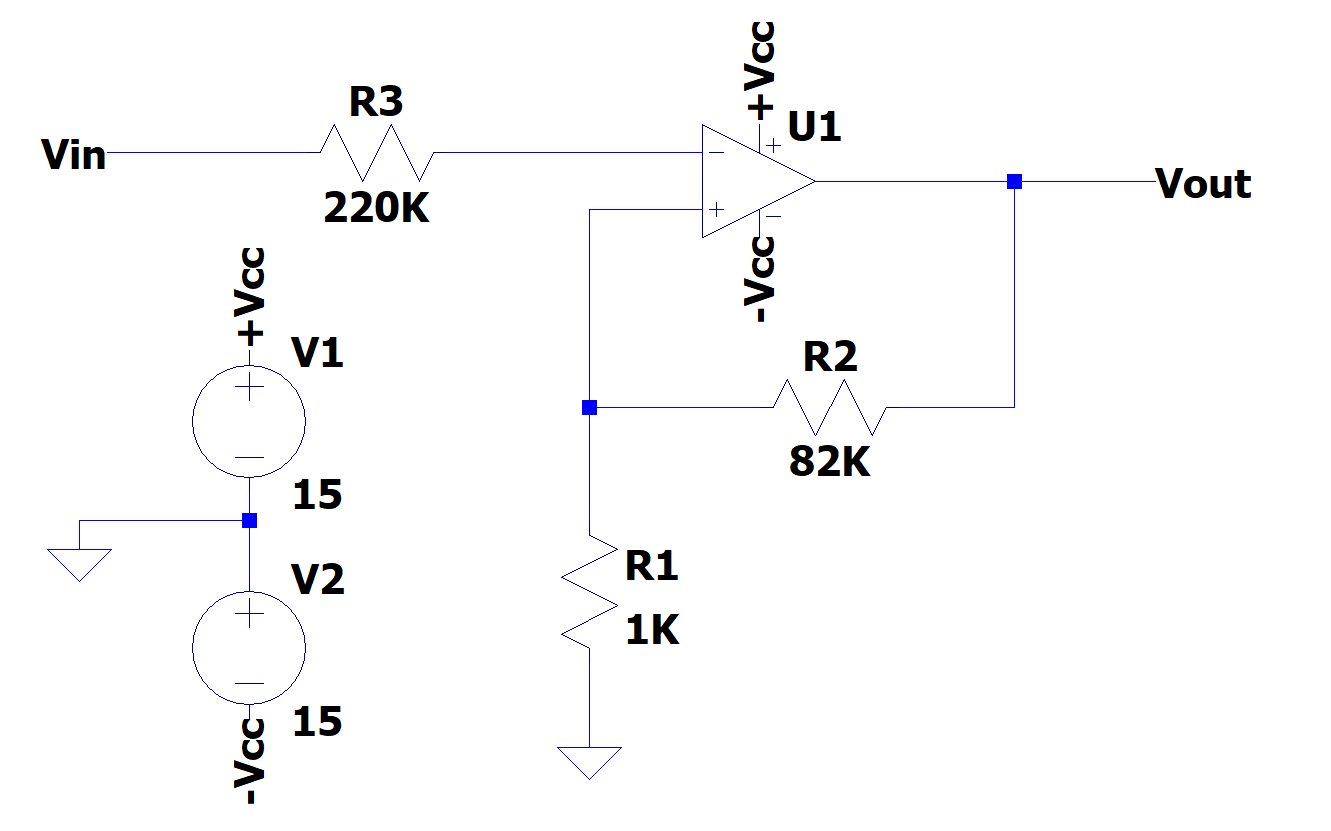
\includegraphics[width=\textwidth]{../EJ2/recursos_para_el_informe/circuito_a_analizar_ideal}
        \caption{Circuito a analizar.}
        \label{fig:initial_circuit}
    \end{minipage}\hfill
\end{figure}

Ha de prestarse especial atención al nodo de la entrada no inversora del operacional.
El mismo se encuentra a alta impedancia, ya que a su izquierda tiene la resistencia de $220K\Omega$, y a su derecha la impedancia interna del operacional (también alta).
Esto lo convierte esencialmente en una antena, susceptible a captar señales de su entorno y, dado que está conectado a un circuito con una alta amplificación (cercana a los 40dB), amplificar esta señal parásita a la salida.\par
Este problema fue afrontado al realizar las mediciones con el operacional LM833 (uno de los dos pedidos), y se ofreció una solución al mismo que será detallada más adelante en las conclusiones del ejercicio.
Luego, para el segundo operacional (NE5534), se decidió reemplazar a la misma por una de inferior valor, y se tomó como criterio hacer uso de la resistencia óptima para la compensación de las corrientes de bias.
El valor para tal resistencia se obtiene de tomar el paralelo entre la resistencia de entrada al sistema, y la de feedback:
\begin{equation}
    R_3' = \frac{R_1 \cdot R_2}{R_1 + R_2} = \frac{1K\Omega \cdot 82K\Omega}{1K\Omega + 82K\Omega} \approx 1K\Omega
\end{equation}

\subsubsection{Modelo ideal}
La primer aproximación al comportamiento del circuito se realizará considerando al amplificador operacional como un componente ideal, es decir, $Av = \inf$, $Z_{in_{opamp}} = \inf$, $Z_{out_{opamp}} = 0$.
De esta manera, sin importar el modelo de operacional utilizado, se tiene que:
\begin{equation}
    \label{eq:ideal_gain}
    \frac{v_{out}}{v_{in}} = 1 + \frac{R_2}{R_1} = 1 + \frac{82 K\Omega}{1 K\Omega} = 83 \implies 38,38 dB
\end{equation}

Se desprende también, de las condiciones de idealidad impuestas, que la impedancia de entrada del circuito será infinita.


\subsubsection{Modelo con impedancia de entrada, salida, y ganancia finita}
Para la resolución del circuito con las consideraciones ya mencionadas, es necesario ahora especificar qué datos serán utilizados para los cálculos.
Los mismos fueron obtenidos de las correspondientes datasheets 
\footnote{Datasheet para operacional LM833: https://www.ti.com/lit/ds/symlink/lm833.pdf \\Datasheet para operacional NE5534: https://www.onsemi.com/pub/Collateral/NE5534-D.PDF}, 
y se presentan en el cuadro \ref{tab:parameters_for_equations}. \par
En particular, para la frecuencia del polo dominante del NE5534, se tomó el dato del polo dominante cuando el capacitor de compensación colocado es de 22pF (el que fue utilizado).
\begin{table}[H]
    \label{tab:parameters_for_equations}
    \centering
    \begin{tabular}{|l|lllll|}
        \hline
        \textbf{\begin{tabular}[c]{@{}l@{}}Modelo de operacional\end{tabular}} & \textbf{\begin{tabular}[c]{@{}l@{}}$f_0$ (Hz)\end{tabular}} & \textbf{\begin{tabular}[c]{@{}l@{}}$A_0$ \end{tabular}} & \textbf{$r_{in_{opamp}}(K\Omega)$} & \textbf{$r_{out_{opamp}}(\Omega)$} & \textbf{$C_{in_{opamp}}(pF)$} \\ \hline
        \textbf{LM833}                                                         & $16 \cdot 10^3$                                             & $1000$                                                  & $175$                              & $37$                               & $12$                          \\
        \textbf{NE5534}                                                        & $1 \cdot 10^3$                                              & $10 \cdot 10^5$                                         & $100$                              & $0,3$                              & -                             \\ \hline
        \end{tabular}
    \caption{Parámetros para cálculo de circuito no ideal.}
\end{table}

Se modelizará al operacional mediante el circuito \ref{fig:non_ideal_circuit}.
\begin{figure}[H]
    \begin{minipage}{\textwidth}
        \centering
        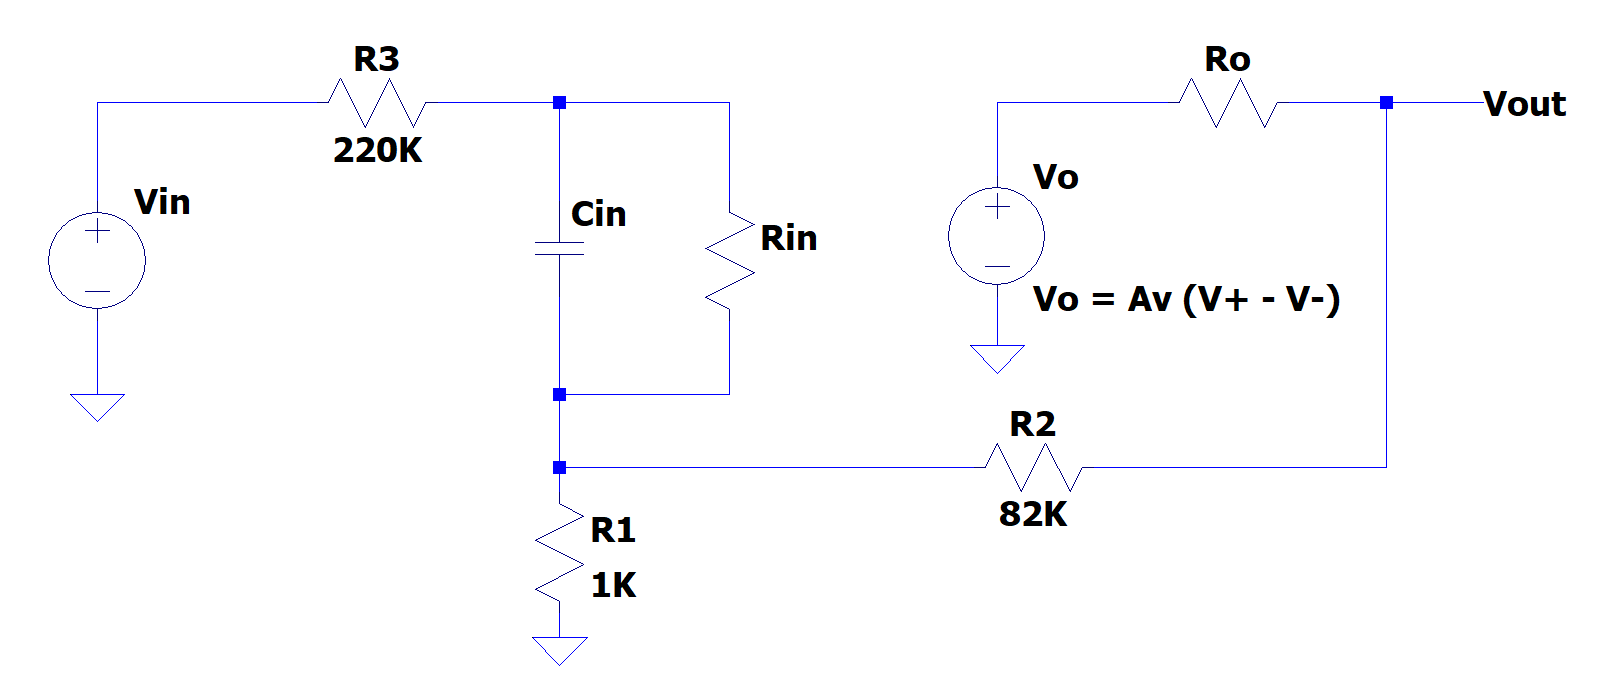
\includegraphics[width=\textwidth]{../EJ2/recursos_para_el_informe/circuito_a_analizar_no_ideal}
        \caption{Circuito a analizar.}
        \label{fig:non_ideal_circuit}
    \end{minipage}\hfill
\end{figure}

Se entiende al circuito como dos mallas cuyas ecuaciones son las descriptas en \ref{eq:system_meshes}, que se extraen del circuito \ref{fig:meshes_circuit}.
\begin{figure}[H]
    \begin{minipage}{\textwidth}
        \centering
        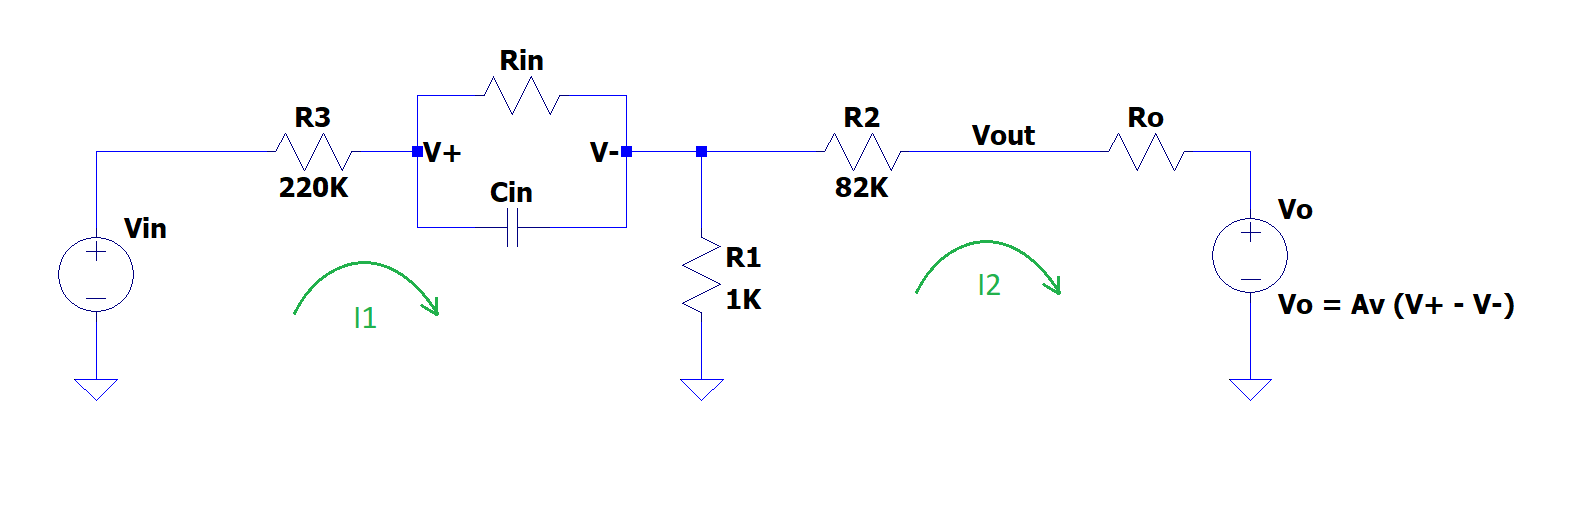
\includegraphics[width=\textwidth]{../EJ2/recursos_para_el_informe/circuito_mallas}
        \caption{Circuito a analizar.}
        \label{fig:meshes_circuit}
    \end{minipage}\hfill
\end{figure}

\begin{align}
    \label{eq:system_meshes}
    &v_{in} - i_1 \cdot R_3 - i_1 \cdot Z_{in} - \left(i_1 - i_2\right) \cdot R_1 = 0 \\
    &-\left(i_2 - i_1\right) \cdot R_1 - i_2 \cdot R_2 - I_2 \cdot R_0 - v_o = 0 \\
    &v_o = \left(v^+ - v^-\right) \cdot A_v \\
    &v^+ = v_{in} - i_1 \cdot R_3 \\
    &v^- = v_{in} - i_1 \cdot R_3 - i_1 \cdot Z_{in} \\
    &Z_{in} = \frac{R_{in}}{R_{in} \cdot C_{in} \cdot s + 1} \label{eq:zin} \\
    &A_v = \frac{A_0}{1+\frac{s}{\omega_p}}
\end{align}

Resolviendo para $i_2$ se obtiene que:
\begin{equation}
    i_2 = v_{in} \cdot \frac{R_1 - A_v \cdot Z_{in}}{R1 \cdot \left(A_v \cdot Z_{in} - R_1\right) + \left(R_3 + Z_{in} + R_1\right) \cdot \left(R_1 + R_2 + R_o\right)}
    \label{eq:i2}
\end{equation}

Y luego se expresan $v_{out}$ e $i_1$ en función de $i_2$ como:
\begin{align}
    \label{eq:i1_and_vout}
    &i_1 = \frac{v_{in} + i_2 \cdot R_1}{R_3 + Z_{in} + R_1} \\
    &v_{out} = v_{in} \cdot \frac{R_1}{R_3 + Z_{in} + R_1} + i_2 \cdot \frac{R_1^2}{R_3 + Z_{in} + R_1} + i_2 \cdot R_1 - i_2 \cdot R_2
\end{align}

\subsubsection{Ecuaciones teóricas para el LM833}
De los resultados obtenidos en \ref{eq:i1_and_vout}, y con los datos de la tabla \ref{tab:parameters_for_equations}, se tiene:
\begin{align}
    & \frac{v_{out}^{LM833}}{v_{in}} = \frac{1,11 \cdot 10^{-4} \cdot s^{4} + 1,105 \cdot 10^{3} \cdot s^{3} + 3,698 \cdot 10^{13} \cdot s^{2} + 3,471b\cdot 10^{20} \cdot s + 2,692 \cdot 10^{26}}
    {s^{4} + 1,034 \cdot 10^{7} s^{3} + 1,678 \cdot 10^{13} \cdot s^{2} + 1,203 \cdot 10^{19} s + 3,948 \cdot 10^{24}} \label{eq:LM833_transfer_fun} \\
    & Z_{in}^{LM833} = \frac{2,21 \cdot 10^{5} \cdot s^3 + 1,89 \cdot 10^{11} \cdot s^2 + 1,49 \cdot 10^{17} \cdot s + 4,12 \cdot 10^{22}}
    {s^3 + 4,78 \cdot 10^{5} \cdot s^2 + 3,79 \cdot 10^{10} \cdot s} \label{eq:LM833_in_impedance} \\
\end{align}
\todo[inline]{NE5534 Transfer function}

\subsubsection{Ecuaciones teóricas para el NE5534}
De los resultados obtenidos en \ref{eq:i1_and_vout}, y con los datos de la tabla \ref{tab:parameters_for_equations}, se tiene:
\begin{align}
    & \frac{v_{out}^{NE5534}}{v_{in}} = \label{eq:NE5534_transfer_fun} \\
    & Z_{in}^{NE5534} = \label{eq:NE5534_in_impedance}
\end{align}
\todo[inline]{LM833 Input inpedance}
\todo[inline]{NE5534 Input inpedance}


\subsection{Simulación}
Para el análisis de los circuitos mediante herramientas de simulación se empleó el programa LTspice, para el cual se realizaron dos esquemáticos, uno para cada uno de los operacionales.
En ambos casos, se simuló la respuesta en frecuencia utilizando la función AC Analysis, y se obtuvieron así los diagramas de bode e impedancia de entrada del sistema, seleccionando las variables pertinentes a observar en el graficador.
A continuación se presentan los circuitos utilizados para tal fin:
\missingfigure{Circuit in LTspice for LM833}
\missingfigure{Circuit in LTspice for NE5534}

\subsection{Resultados y comparación}
\subsubsection{Con operacional LM833}
Para realizar las mediciones con este operacional, se decidió buscar la forma de paliar los efectos de la resistencia de $220K\Omega$ mediante el uso de un cable cercano a la misma, y conectado a tierra.
Este cable hace las veces de shield, al ofrecerle a las señales parásitas un camino de menor esfuerzo hacia tierra. \par
Se presentan a continuación los gráficos para la comparación de los resultados teóricos, simulados y experimentales, correspondientes a los diagramas de bode (en módulo y fase), e impedancia de entrada (también en módulo y fase):
\begin{figure}[H]
    \begin{minipage}{\textwidth}
        \centering
        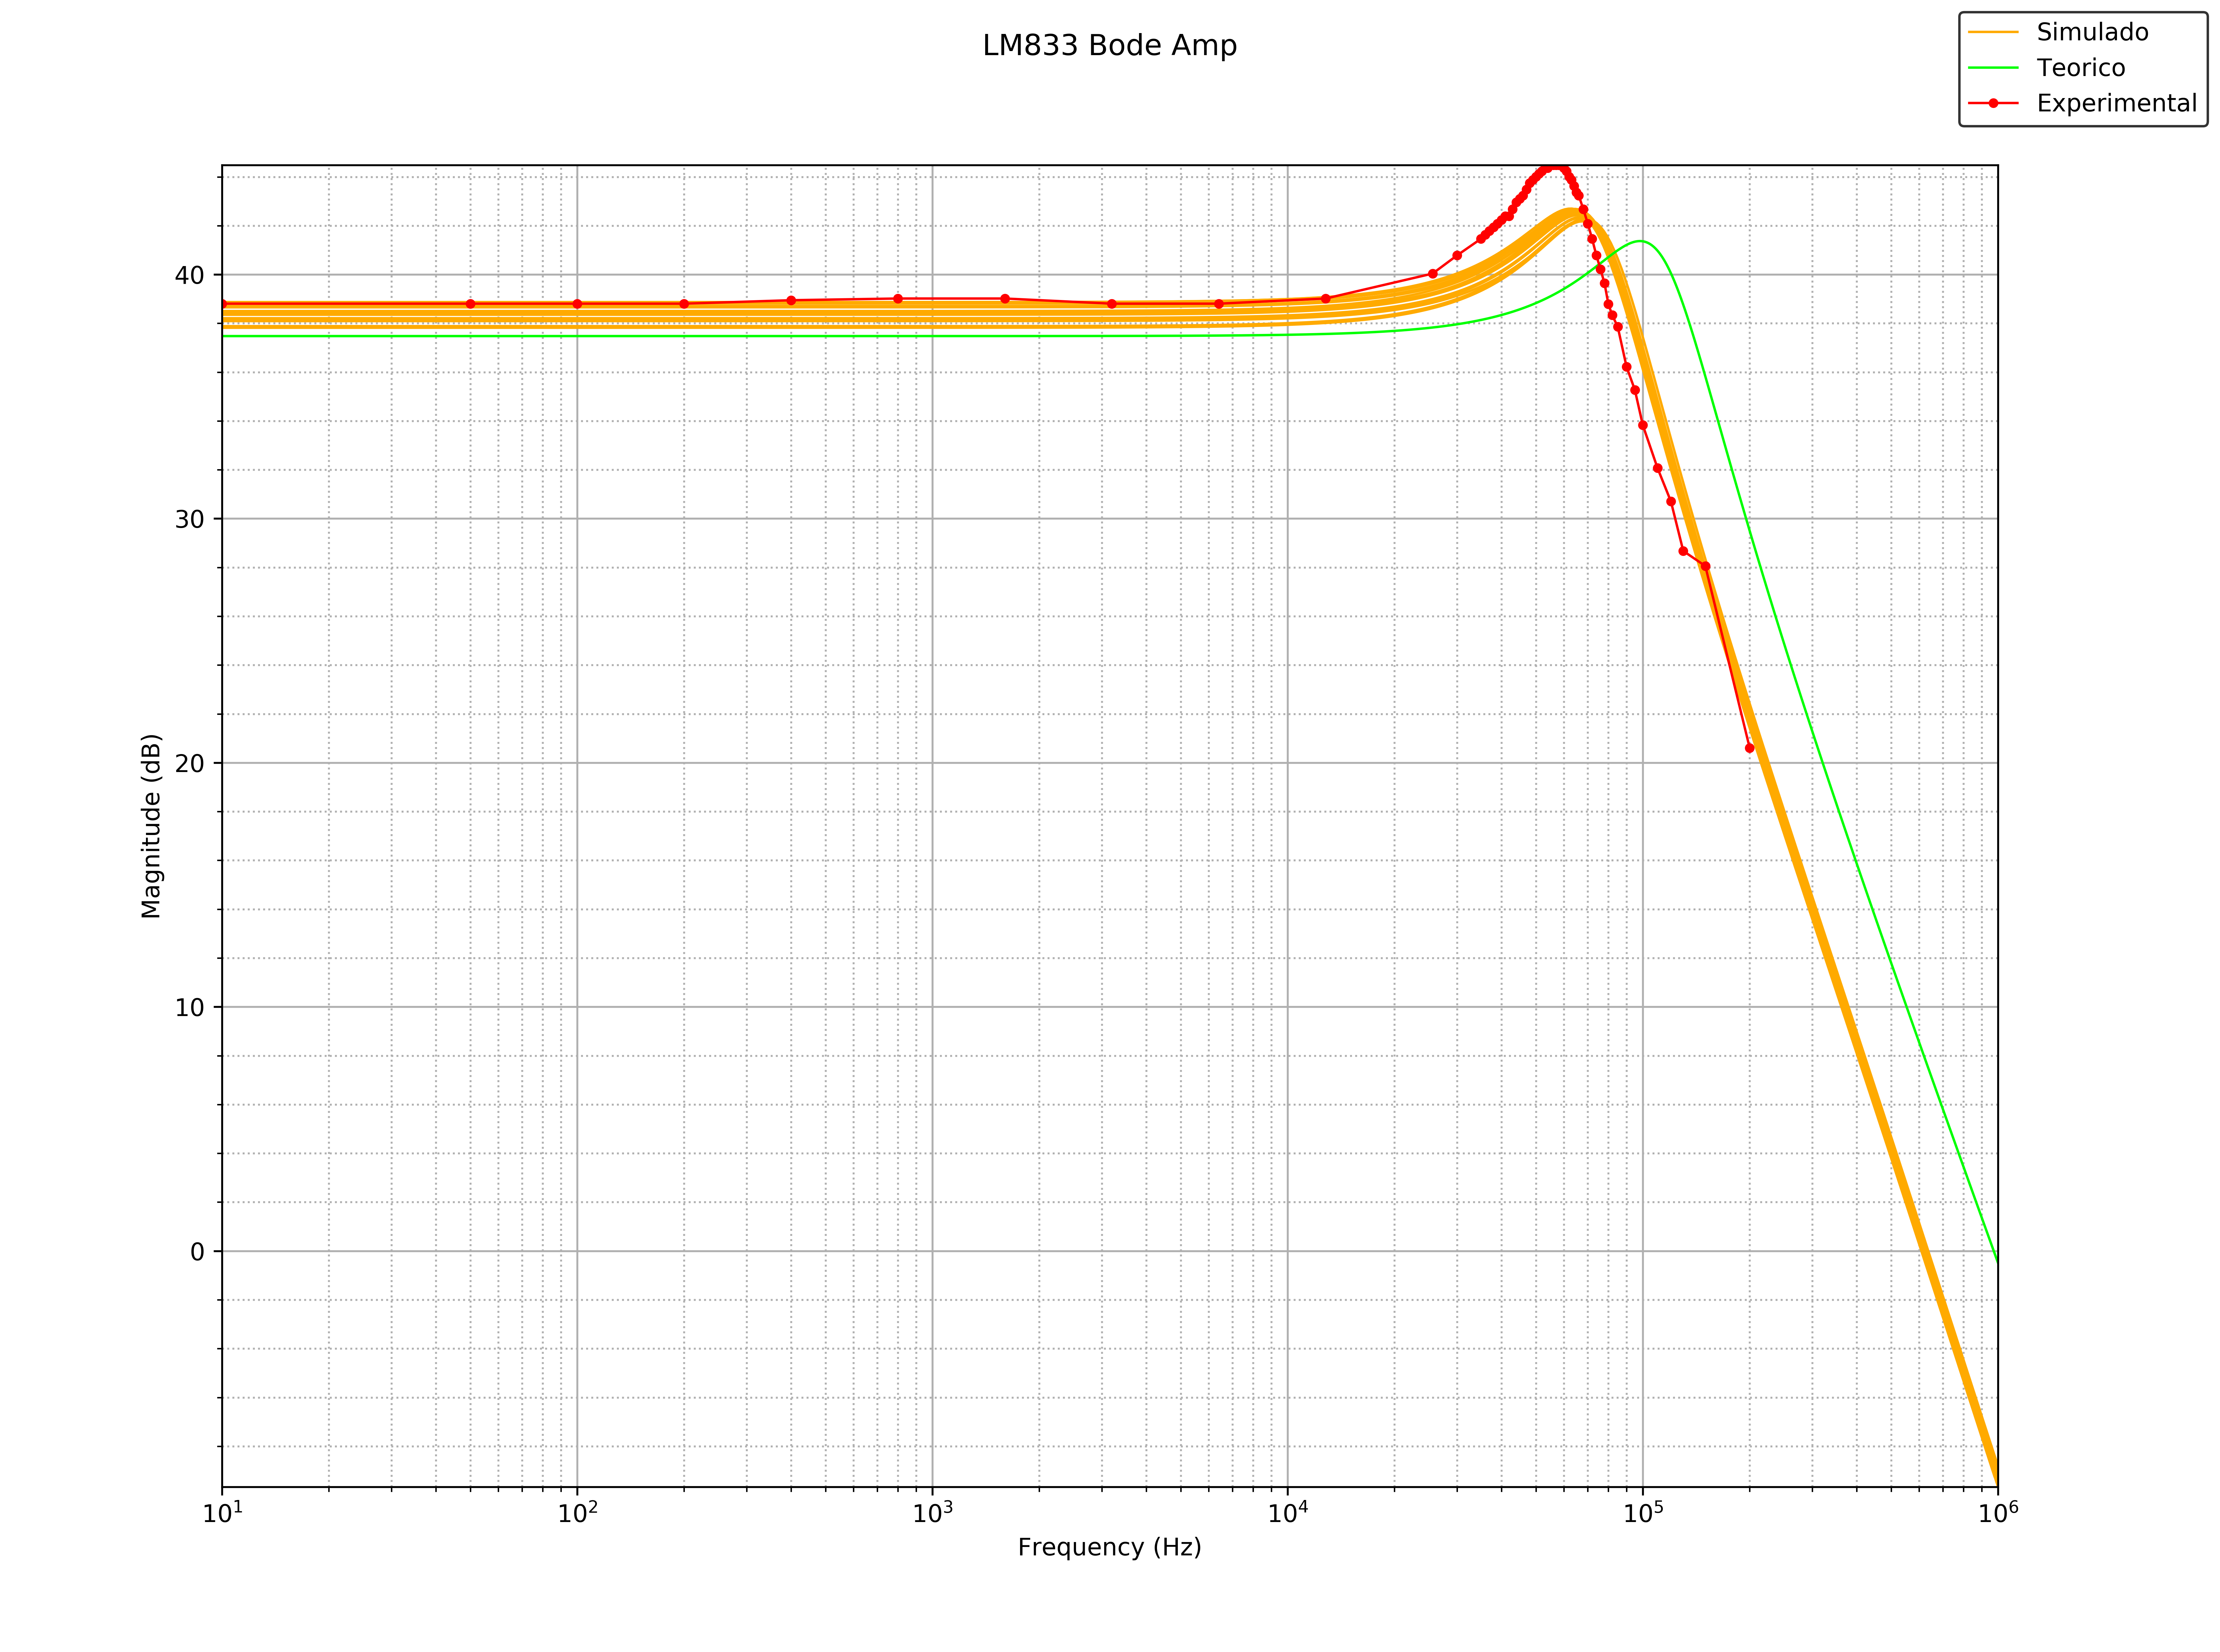
\includegraphics[width=0.8\textwidth]{../EJ2/recursos_para_el_informe/LM833_Bode_Amp}
        \caption{Bode de amplitud para operacional LM833.}
        \label{fig:LM833_Bode_Amp}
    \end{minipage}\hfill
\end{figure}
\begin{figure}[H]
    \begin{minipage}{\textwidth}
        \centering
        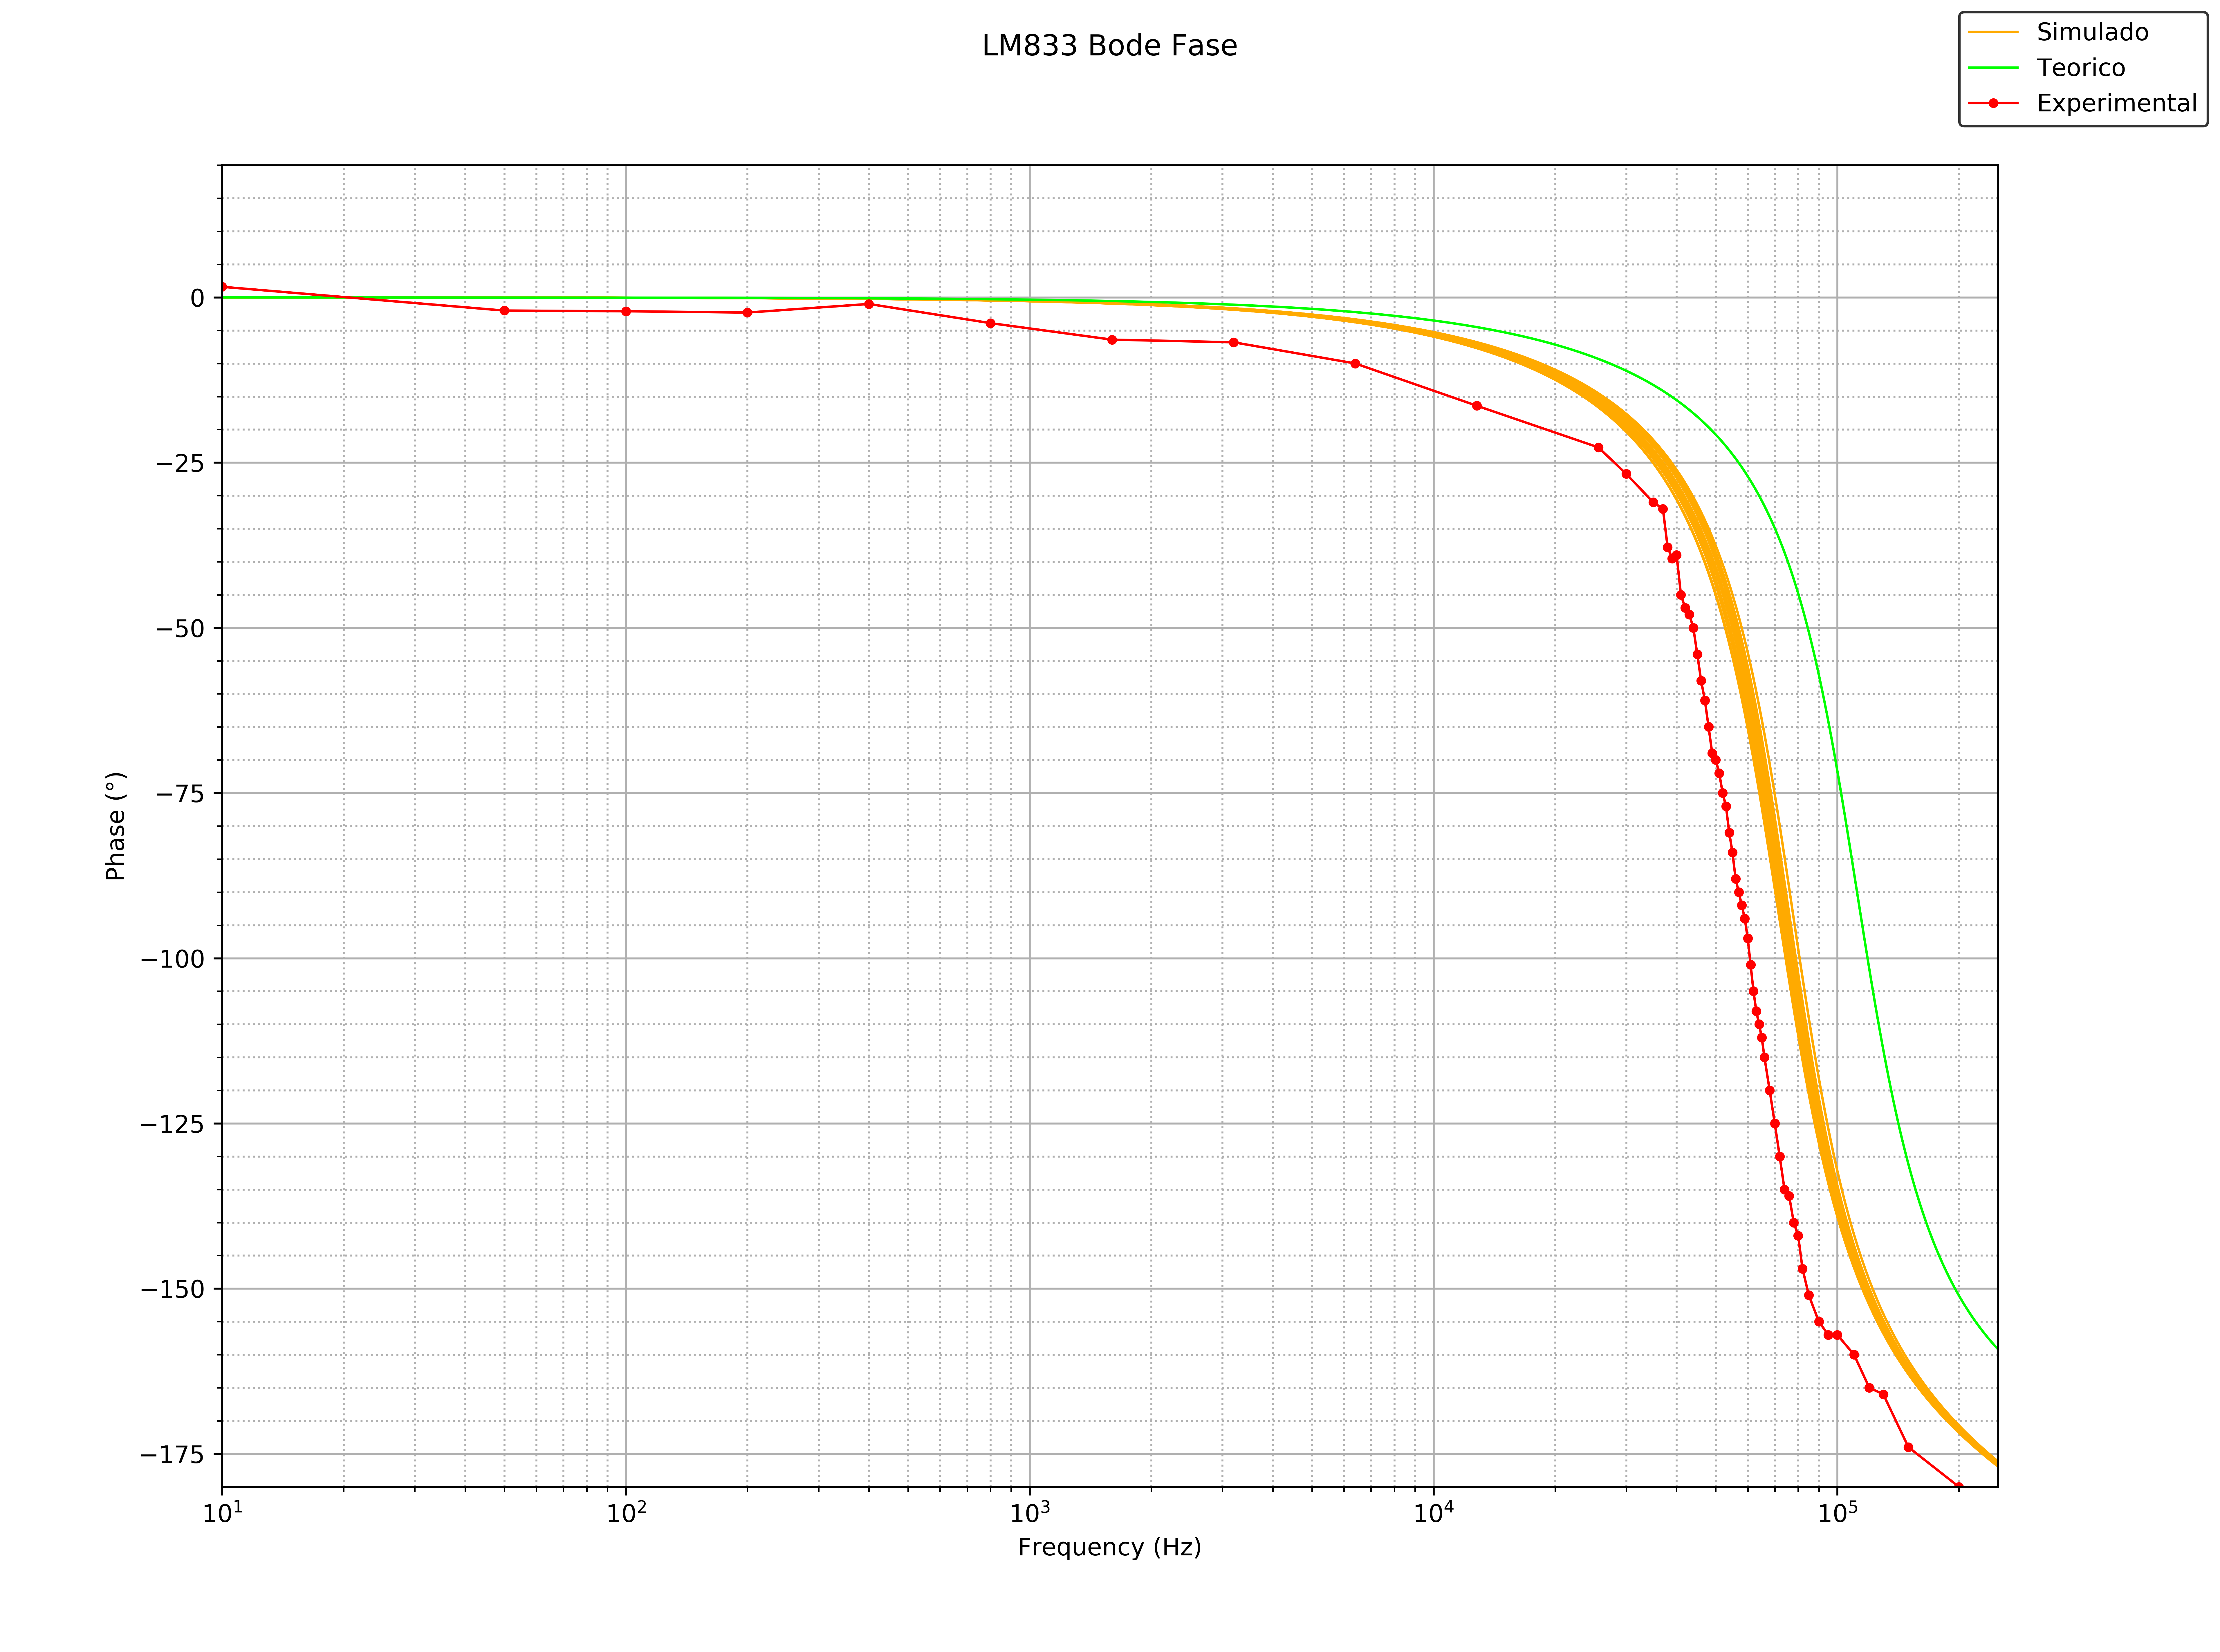
\includegraphics[width=0.8\textwidth]{../EJ2/recursos_para_el_informe/LM833_Bode_Fase}
        \caption{Bode de fase para operacional LM833.}
        \label{fig:LM833_Bode_Fase}
    \end{minipage}\hfill
\end{figure}

Los diagramas de bode se presentan con buena concordancia entre teoría, simulación y práctica, observándose únicamente discrepancias en la frecuencia exacta de corte, y en la magnitud del sobrepico.
Tanto en la amplitud como la fase, se observa una diferencia de aproximadamente 50KHz entre la frecuencia de corte del teórico y del simulado, y otros 10KHz con el medido.
En lo que respecta al sobrepico, el teórico se encuentra en 41dB aproximadamente, mientras que el simulado es de 42, y el medido de 44.
Por otro lado, se observa una coincidencia en la pendiente decreciente posterior al polo, siendo la misma de 40dB por década en las tres curvas.
Esto, sumado 
\begin{figure}[H]
    \begin{minipage}{\textwidth}
        \centering
        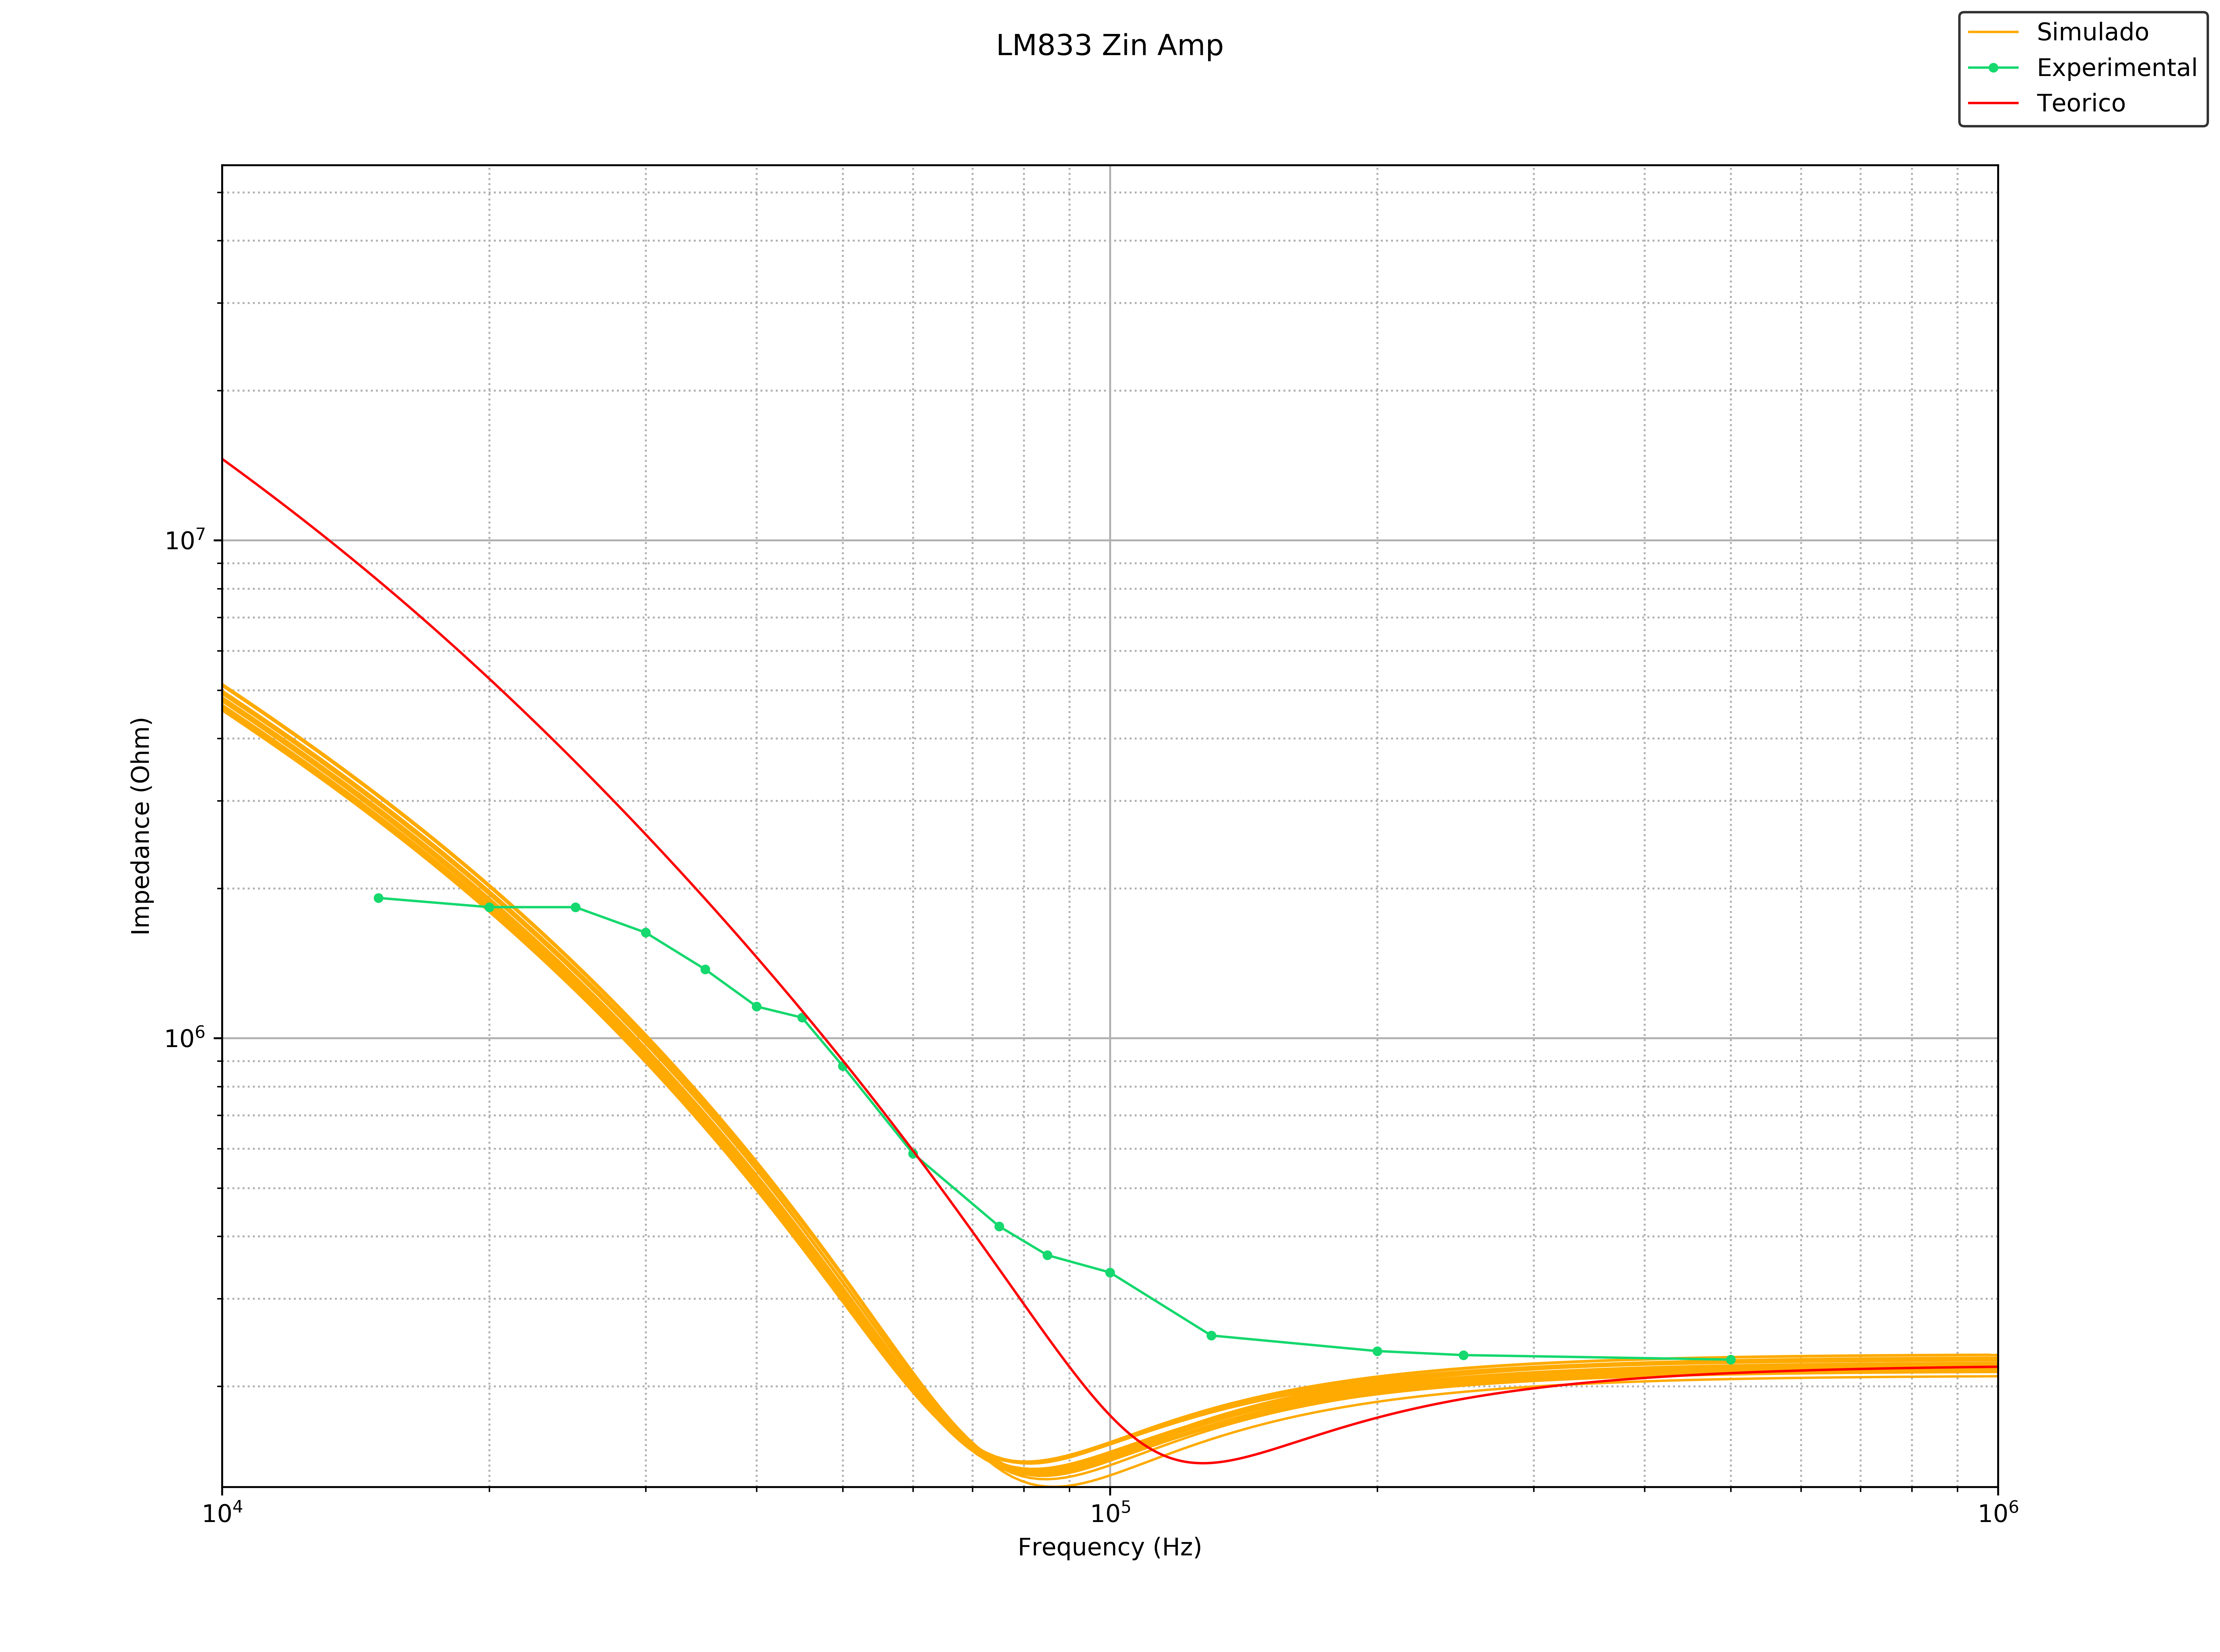
\includegraphics[width=0.8\textwidth]{../EJ2/recursos_para_el_informe/LM833_Zin_Amp}
        \caption{Amplitud de $Z_{in}$ para operacional LM833.}
        \label{fig:LM833_Zin_Amp}
    \end{minipage}\hfill
\end{figure}
\begin{figure}[H]
    \begin{minipage}{\textwidth}
        \centering
        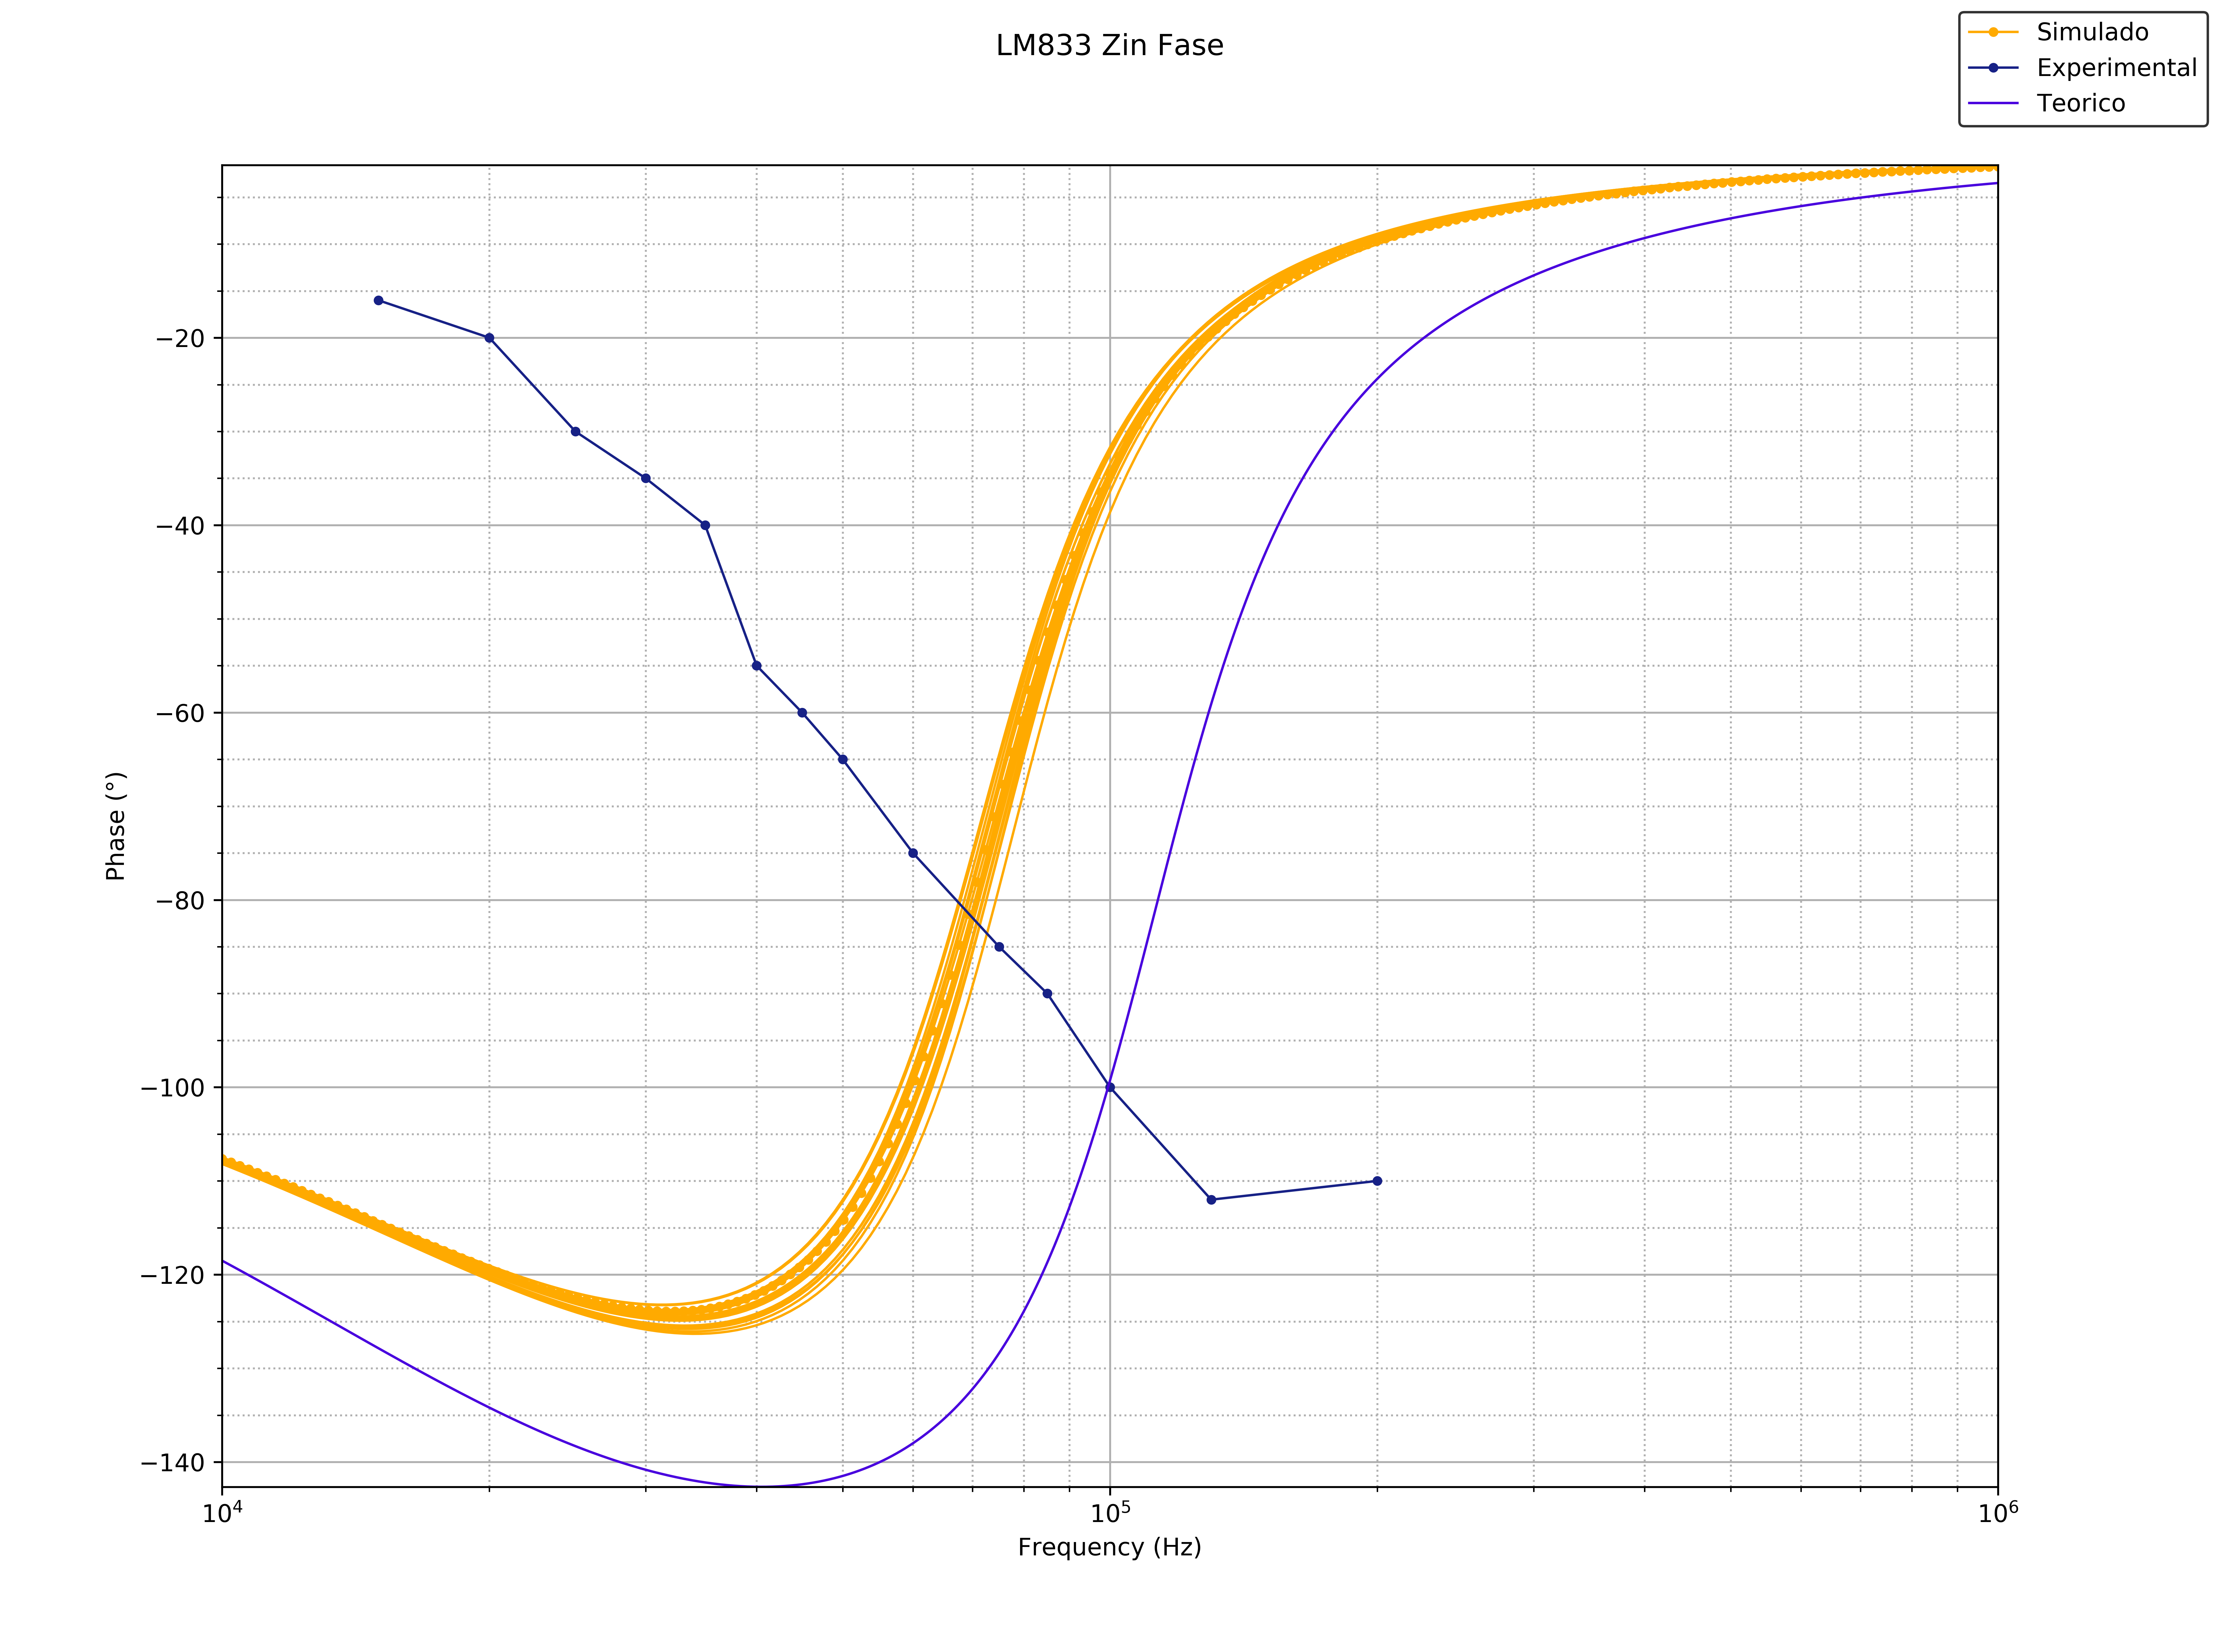
\includegraphics[width=0.8\textwidth]{../EJ2/recursos_para_el_informe/LM833_Zin_Fase}
        \caption{Fase de $Z_{in}$ para operacional LM833.}
        \label{fig:LM833_Zin_Fase}
    \end{minipage}\hfill
\end{figure}

El caso es distinto para la impedancia de entrada, donde las discrepancias son más apreciables.
Mientras que la teoría y la práctica mantienen cierta concordancia, a pesar de su desplazamiento relativo, los valores medidos están en desacuerdo con lo esperado, ya que no presentan el mínimo que caracteriza al teórico y simulado, y en frecuencias donde la fase teórica y simulada crece acercándose al 0, en la práctica decrece. \par
Las razones detrás de estas diferencias pueden estar debidas a las condiciones a las que el circuito fue sometido.
Cabe recordar que a la entrada del mismo se colocó una resistencia de un valor descomunalmente alto para esta aplicación ($220K\Omega$), que es susceptible a captar señales rondantes al mismo.
Esta característica, sumada al hecho de que se está requiriendo una alta amplificación por parte del circuito (cercana a 40dB), contribuyen a que el mismo se encuentre en condiciones excepcionales y límite.
En estas condiciones, es posible que aparezcan efectos en el operacional que no fueron considerados en el análisis teórico ni agregados en el modelo de spice, o que por el contrario, las mediciones hayan carecido de exactitud, siendo más permeables al ruido.



\subsubsection{Con operacional NE5534}
Para las mediciones con este operacional, se decidió dejar de lado la resistencia de $220K\Omega$, y reemplazarla por $1K\Omega$, bajo el criterio mencionado en la sección \ref{sec:ej2_initial}. \par
Se presentan a continuación los gráficos para la comparación de los resultados teóricos, simulados y experimentales, correspondientes a los diagramas de bode (en módulo y fase), e impedancia de entrada (también en módulo y fase):
\begin{figure}[H]
    \begin{minipage}{\textwidth}
        \centering
        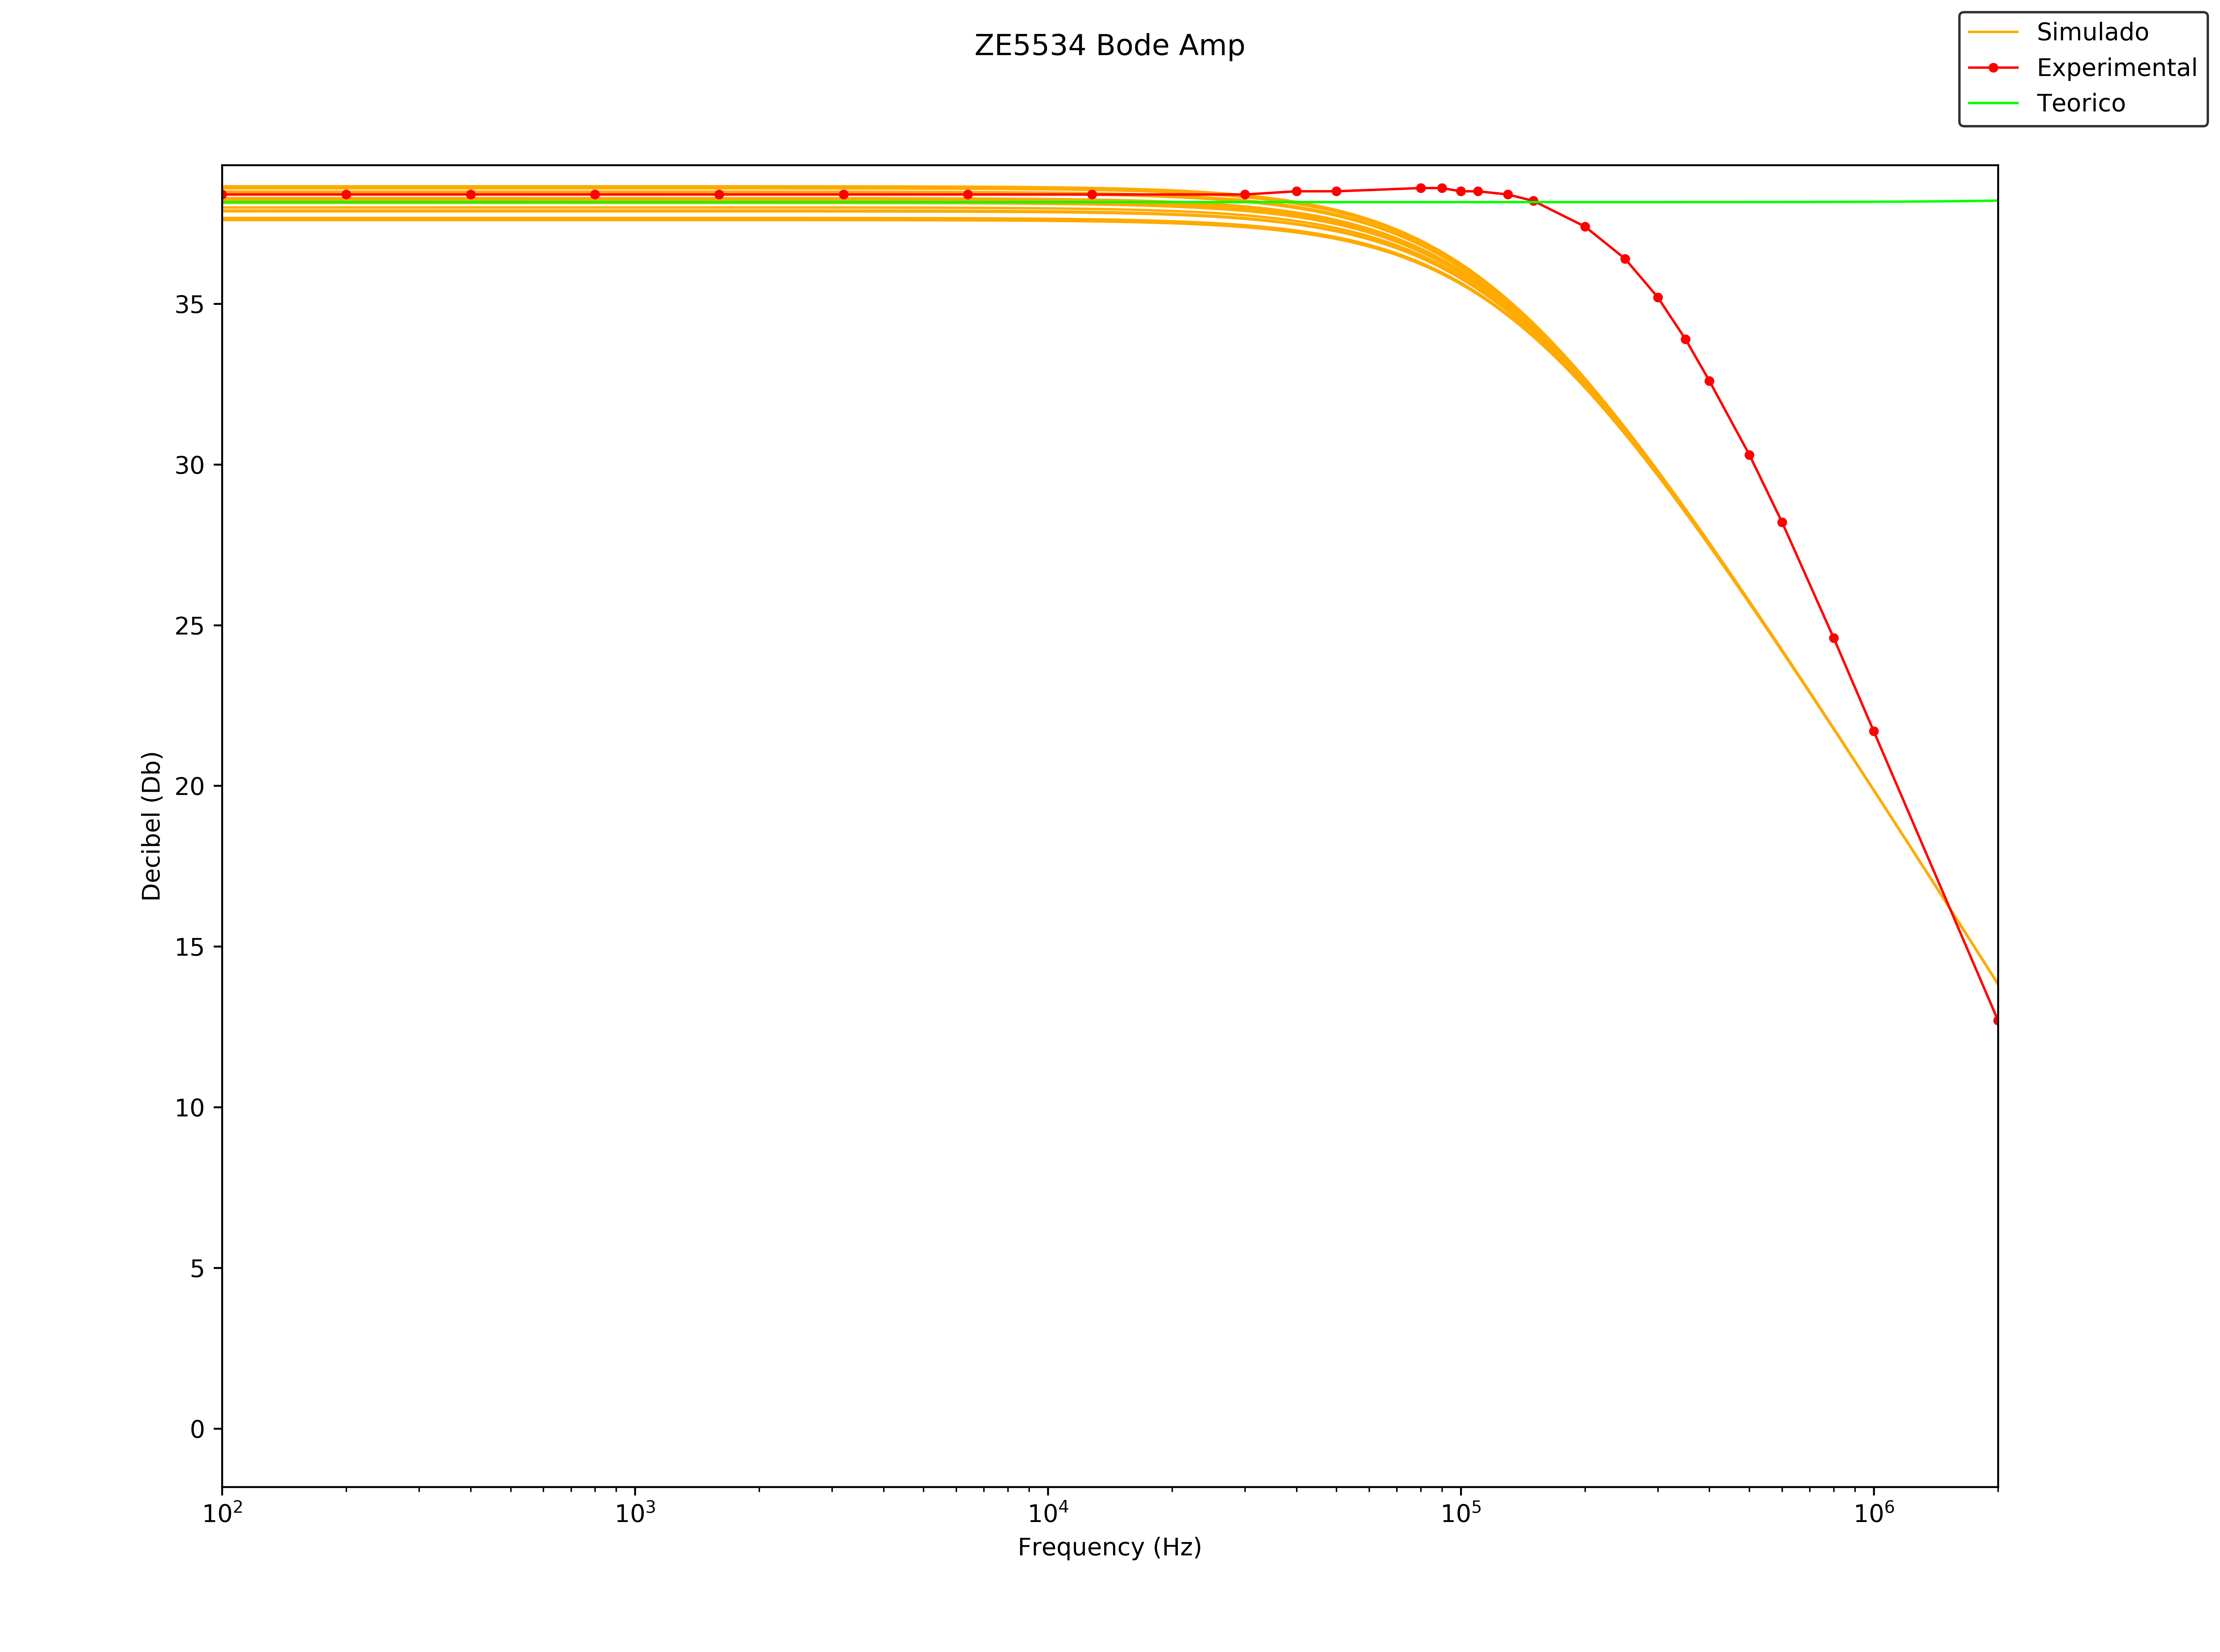
\includegraphics[width=0.8\textwidth]{../EJ2/recursos_para_el_informe/NE5534_Bode_Amp}
        \caption{Bode de amplitud para operacional NE5534.}
        \label{fig:NE5534_Bode_Amp}
    \end{minipage}\hfill
\end{figure}
\begin{figure}[H]
    \begin{minipage}{\textwidth}
        \centering
        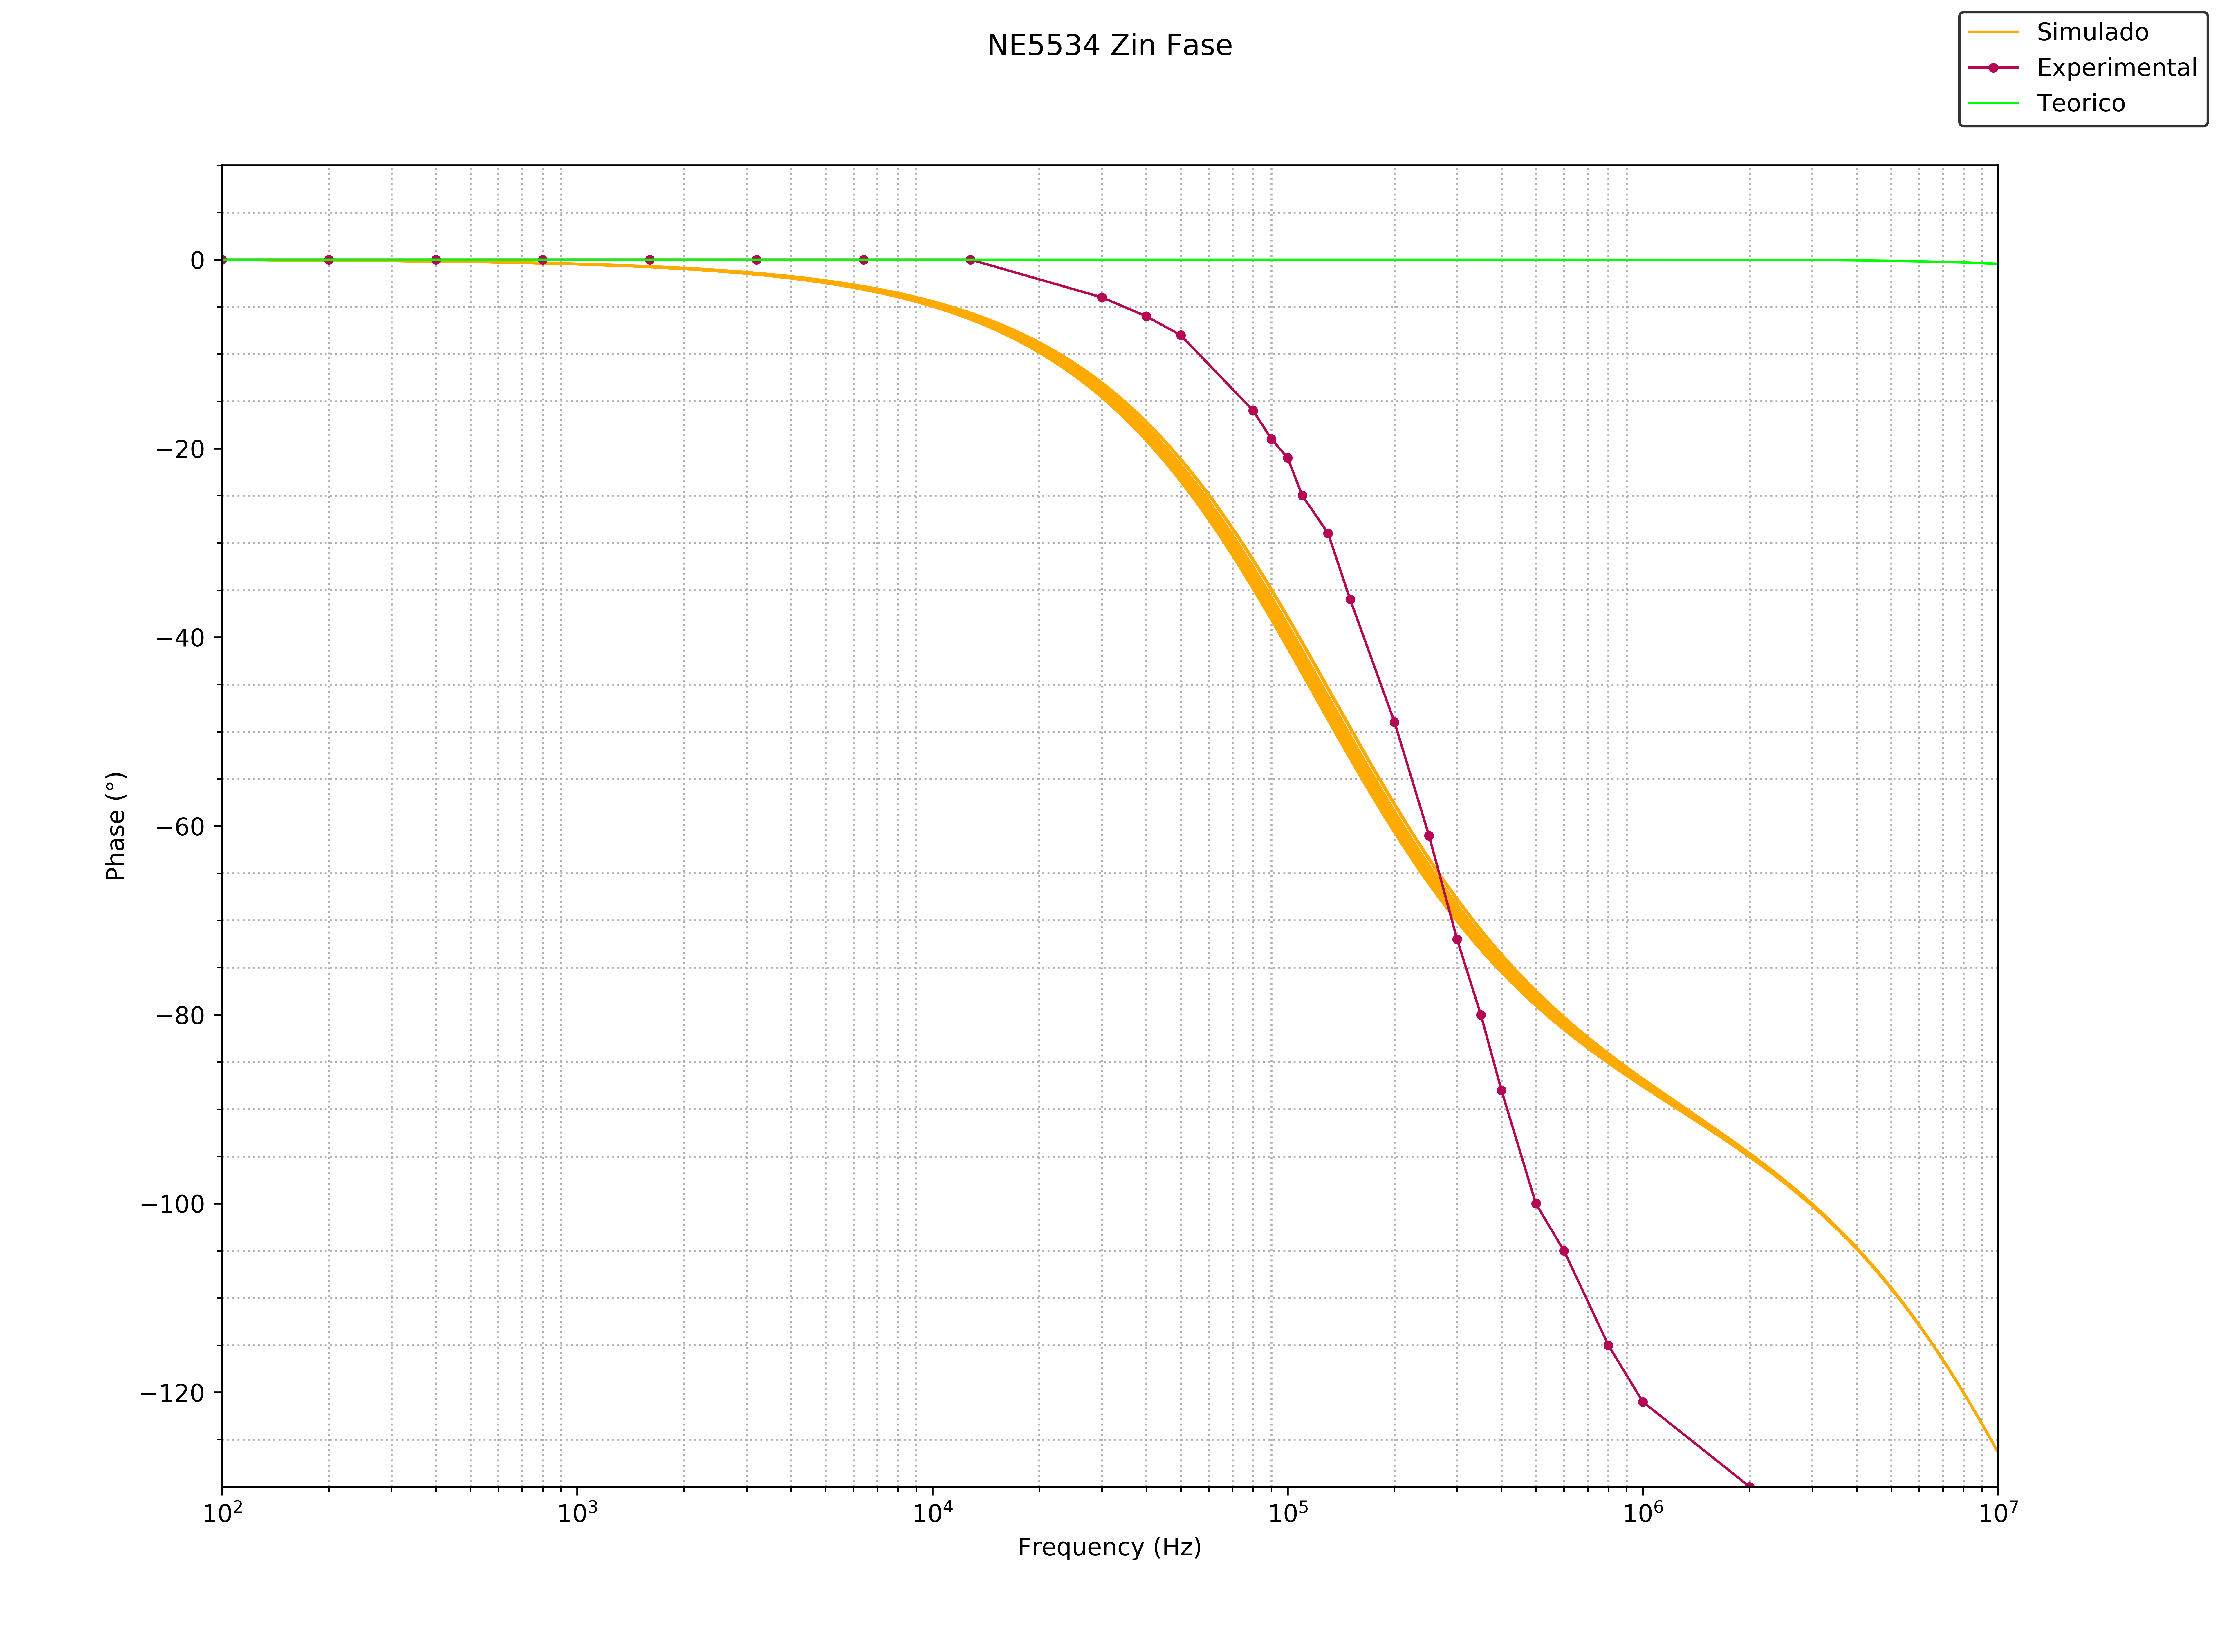
\includegraphics[width=0.8\textwidth]{../EJ2/recursos_para_el_informe/NE5534_Bode_Fase}
        \caption{Bode de fase para operacional NE5534.}
        \label{fig:NE5534_Bode_Fase}
    \end{minipage}\hfill
\end{figure}

El análisis de los resultados de las mediciones con el operacional NE5534 presenta mayores diferencias entre valores prácticos, teóricos e incluso simulados.
En primer lugar, debe ser señalado que el teórico no se realizó teniendo en cuenta la compensación externa con el capacitor de 22pF, razón por la cual se ve que mantiene la ganancia ideal en un ancho de banda mucho más amplio.
En cuanto a la comparación entre el simulado y el experimental, hay una característica fundamental a destacar, y es que la pendiente de decrecimiento de la curva experimental es claramente superior a la simulada, indicando la posible presencia de un polo de segundo orden en lugar de uno simple como sugiere la simulación.
A esto se suma un leve sobrepico que presentan los resultados prácticos, sugiriendo que además de ser de segundo órden, el polo es levemente subamortiguado.
La hipótesis del polo de segundo órden parece ser confirmada en el diagrama de la fase, en el cual se puede observar que mientras que la simulación presenta un cambio de fase de 90°, la experimental salta 180°.
\begin{figure}[H]
    \begin{minipage}{\textwidth}
        \centering
        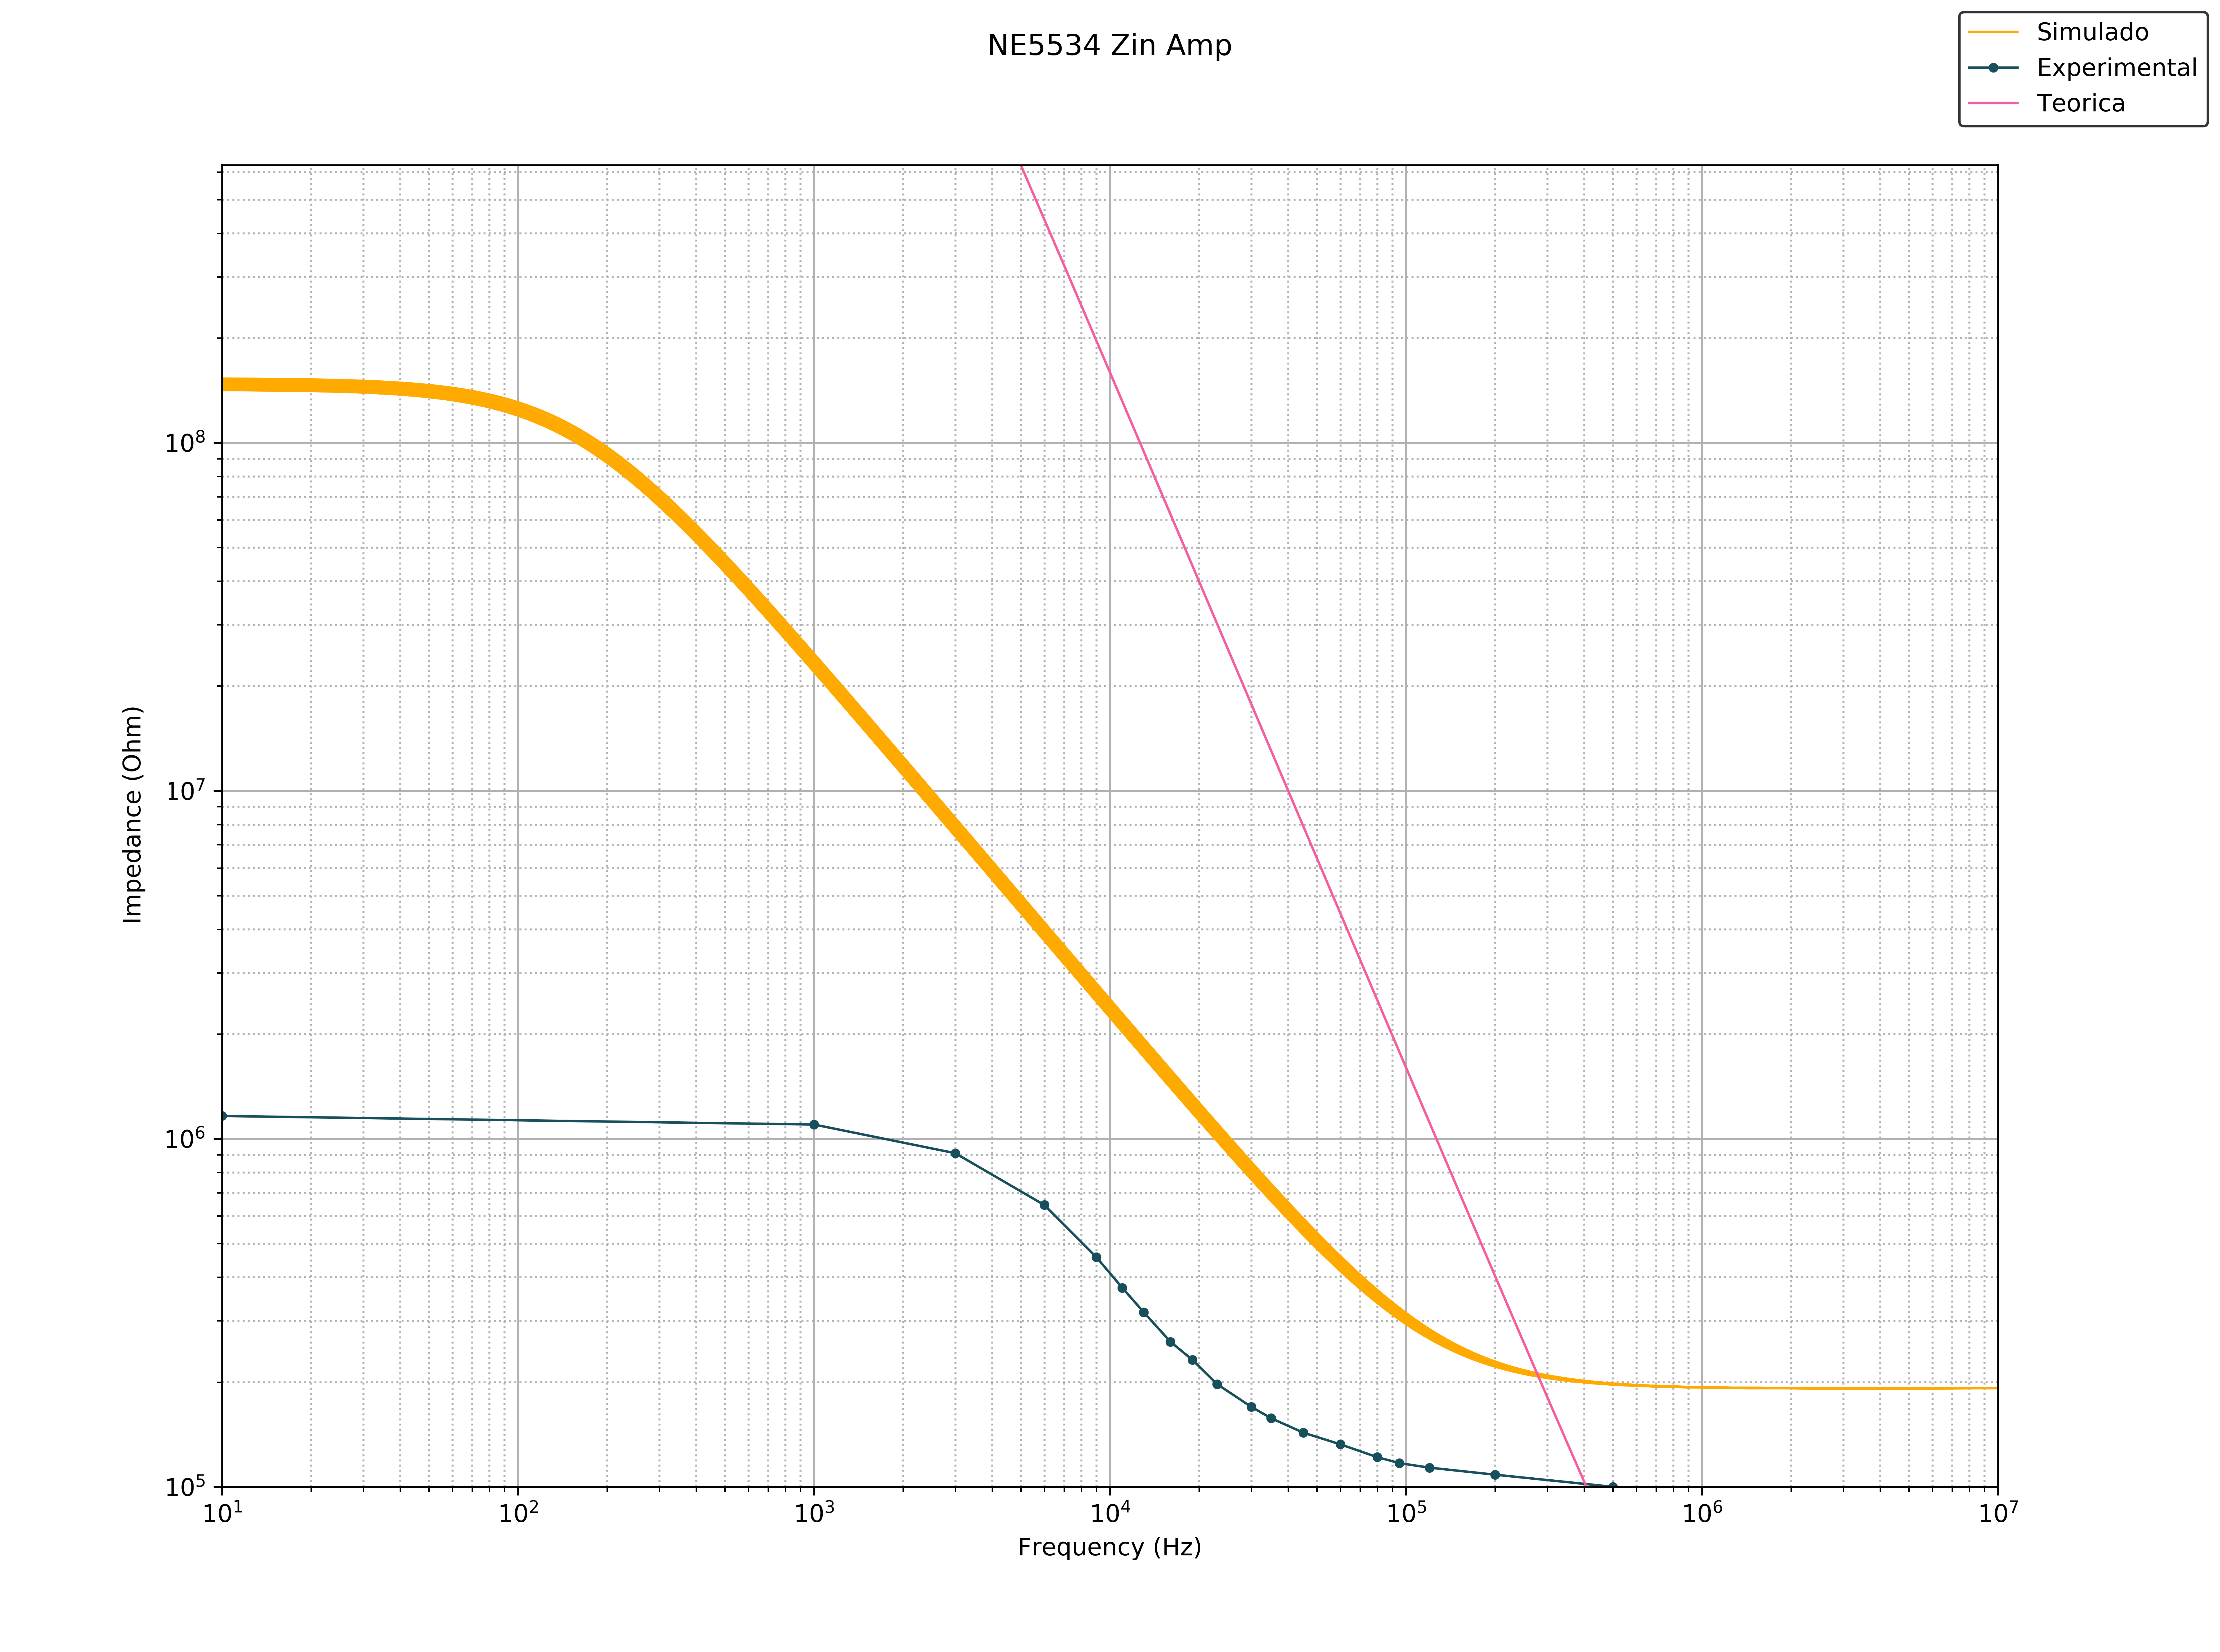
\includegraphics[width=0.8\textwidth]{../EJ2/recursos_para_el_informe/NE5534_Zin_Amp}
        \caption{Amplitud de $Z_{in}$ para operacional NE5534.}
        \label{fig:NE5534_Zin_Amp}
    \end{minipage}\hfill
\end{figure}
\begin{figure}[H]
    \begin{minipage}{\textwidth}
        \centering
        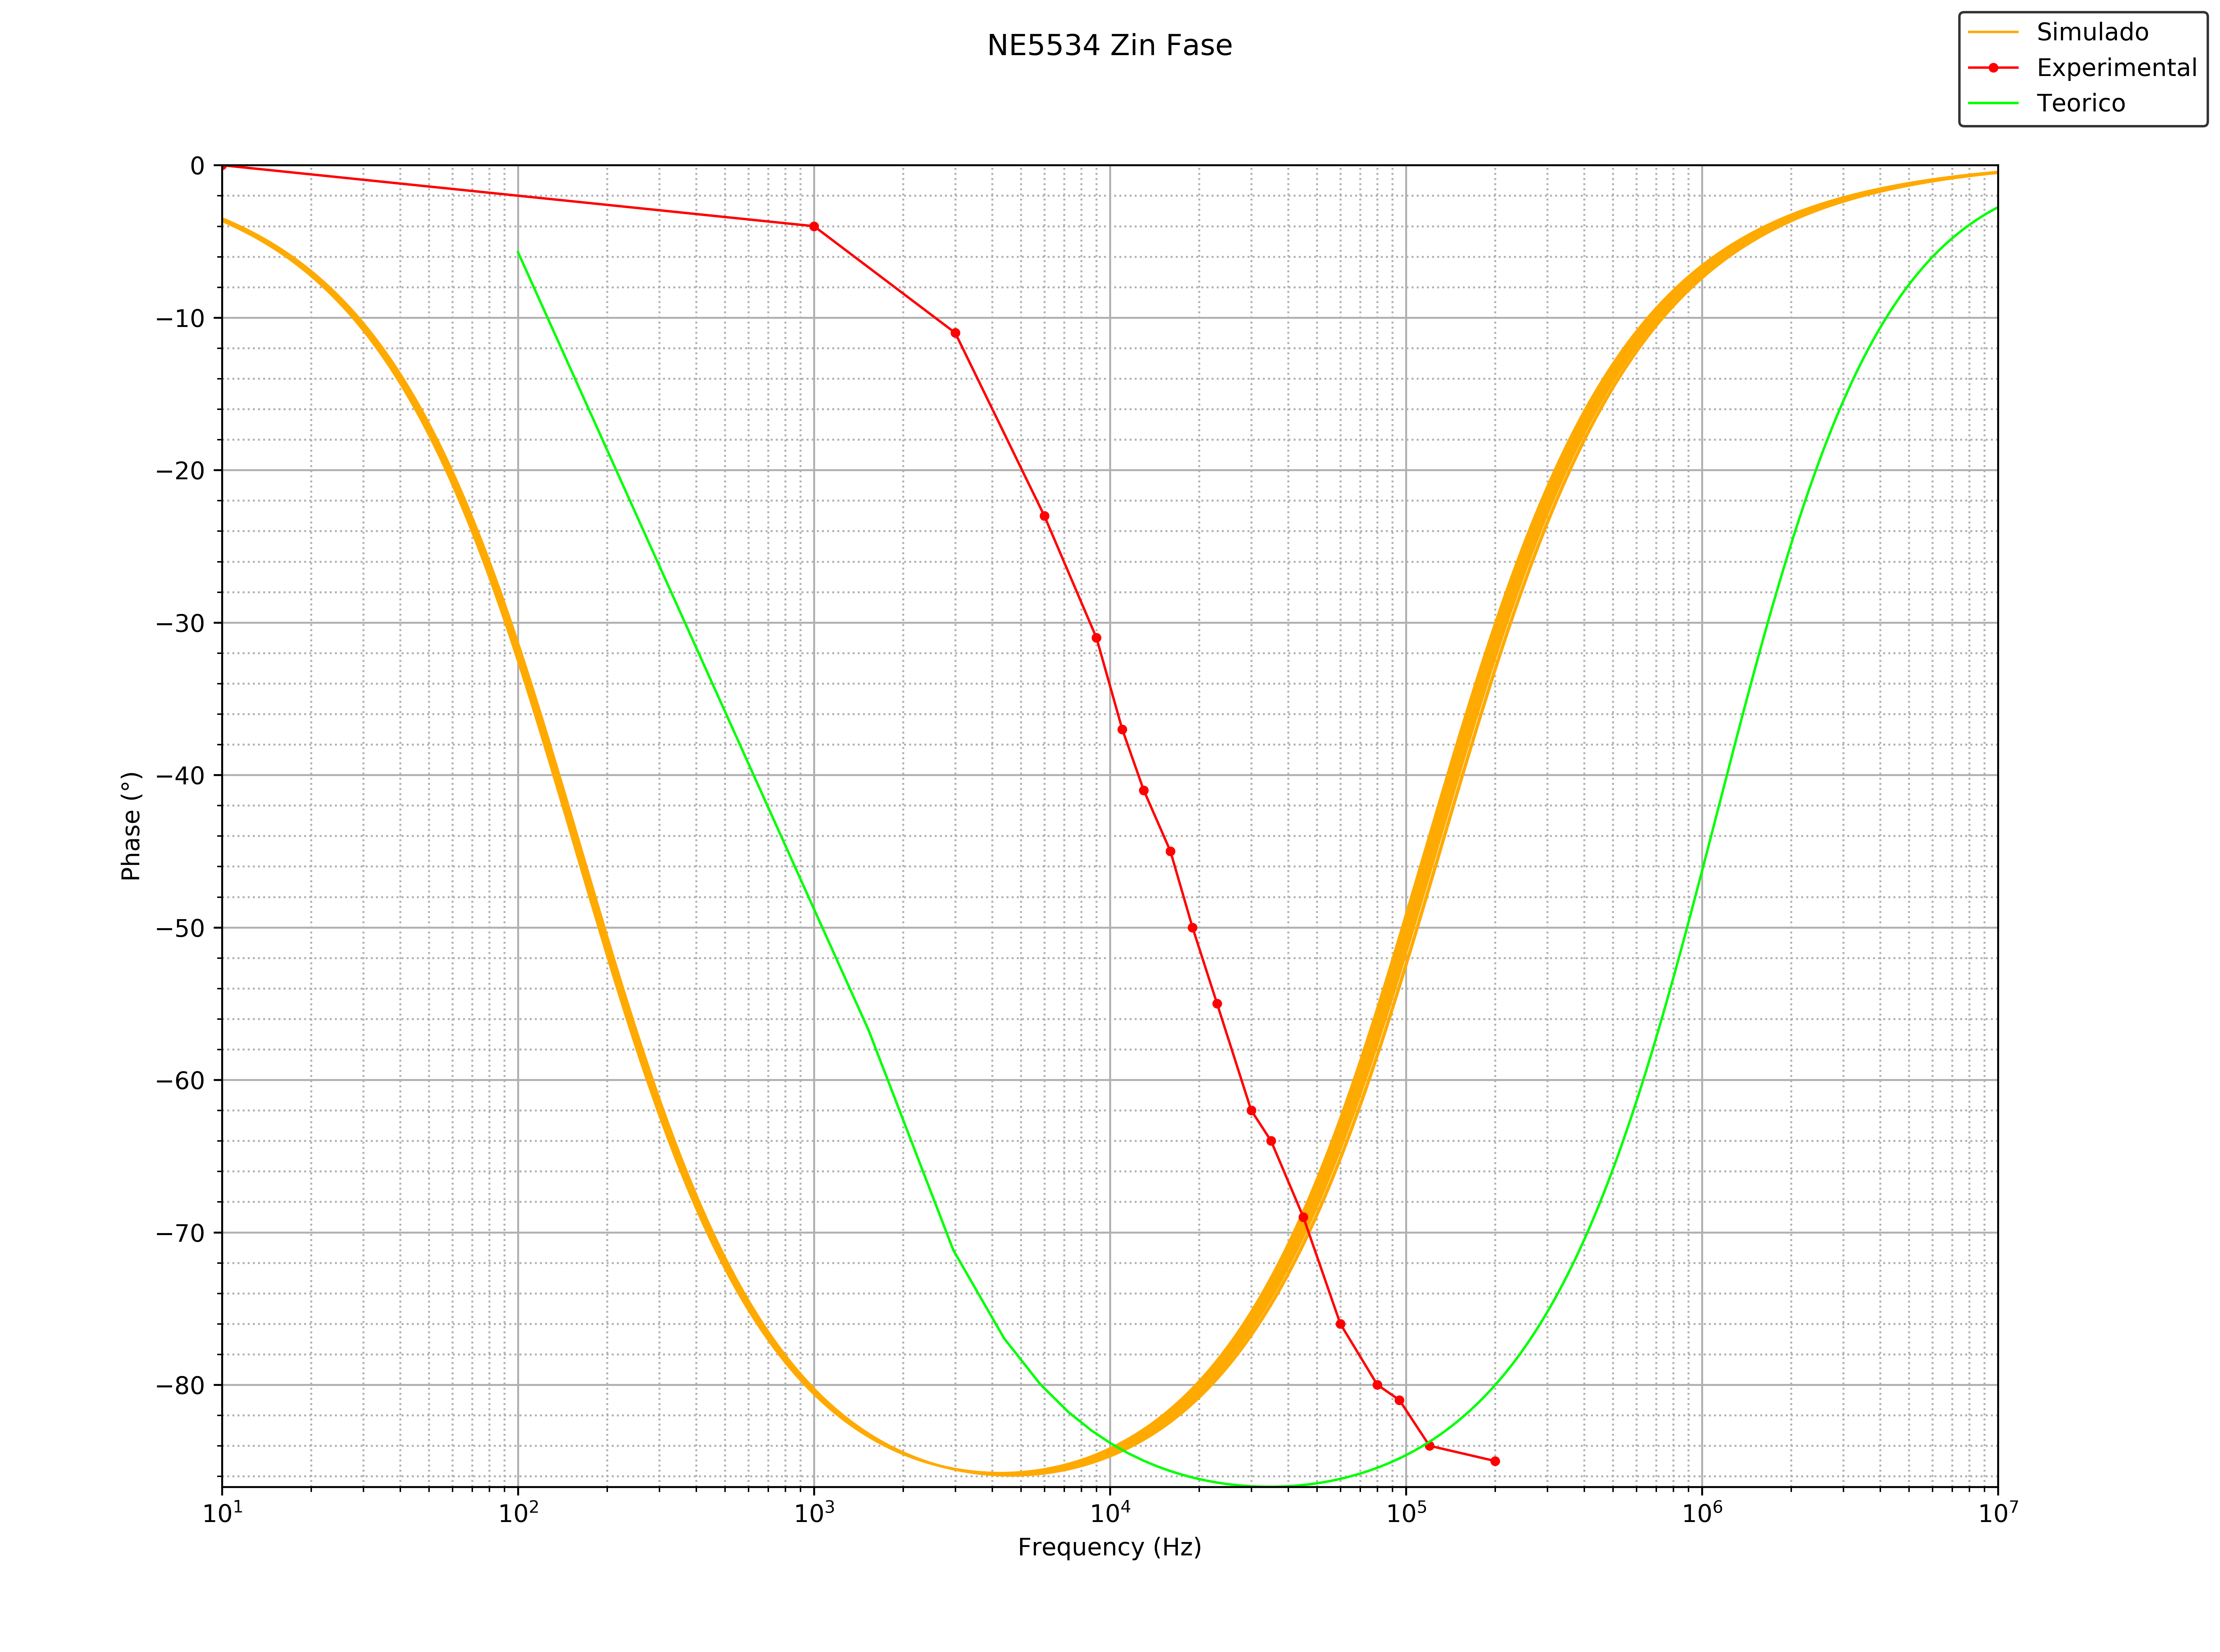
\includegraphics[width=0.8\textwidth]{../EJ2/recursos_para_el_informe/NE5534_Zin_Fase}
        \caption{Fase de $Z_{in}$ para operacional NE5534.}
        \label{fig:NE5534_Zin_Fase}
    \end{minipage}\hfill
\end{figure}

En la impedancia de entrada del NE5534, las diferencias entre las tres curvas se vuelven considerables.
Estas diferencias pueden ser debidas, en parte, a lo señalado por los diagramas de bode, y a las condiciones extremas de uso de un operacional con pobres características.
El NE5534 tiene una baja impedancia de entrada ($100K\Omega$), para una aplicación con tanta ganancia (40dB), y considerando además que ni la teoría ni la simulación tuvieron en cuenta algún componente del operacional que provoca el segundo orden en el polo, puede entenderse entonces que hayan diferencias.
De todas maneras, se concluye que el análisis previo a las mediciones no fue suficiente para predecir los efectos que se presentaron en la práctica.



\subsection{Conclusiones}
De lo visto en este ejercicio se extraen principalmente los conocimientos construidos a partir de los problemas ocasionados por la alta resistencia a la entrada.
Se concluye que es necesario prestar atención a altas impedancias en el nodo de entrada del operacional, ya que convierte al mismo en una antena.
En estas condiciones, y dependiendo del layout del circuito, el mismo puede ser sometido a señales que lo hagan saturar y oscilar.
Finalmente, sobre los operacionales utilizados, se considera que no son recomendables para aplicaciones con tan alta ganancia, particularmente el NE5534, ya que además de requerir una compensación externa, presenta efectos no esperados como un polo de segundo orden.